\begin{teaserfigure}
    \centering
    \begin{subfigure}{0.25\linewidth}
        \centering
        \begin{adjustbox}{height=.9\textwidth}
            % This file was created by tikzplotlib v0.9.5.
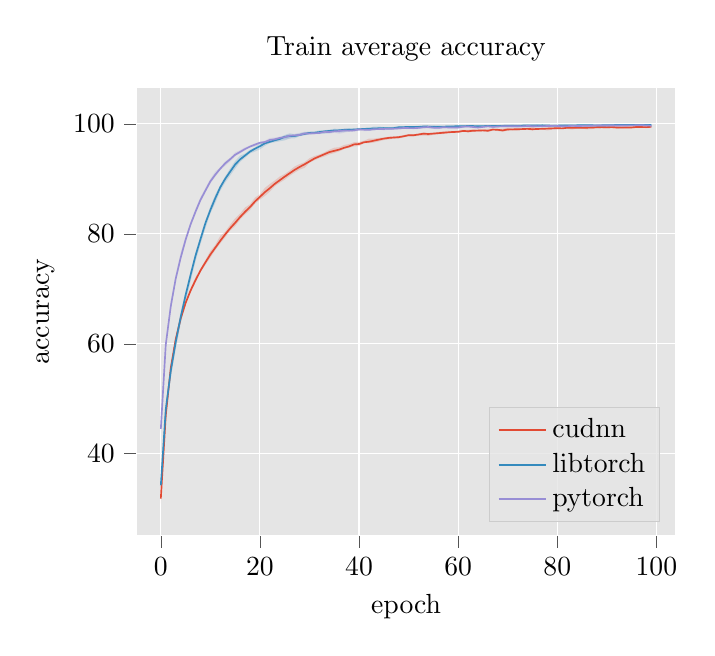
\begin{tikzpicture}

  \definecolor{color0}{rgb}{0.886274509803922,0.290196078431373,0.2}
  \definecolor{color1}{rgb}{0.203921568627451,0.541176470588235,0.741176470588235}
  \definecolor{color2}{rgb}{0.596078431372549,0.556862745098039,0.835294117647059}

  \begin{axis}[
      axis background/.style={fill=white!89.8039215686275!black},
      axis line style={white},
      legend cell align={left},
      legend style={fill opacity=0.8, draw opacity=1, text opacity=1, at={(0.97,0.03)}, anchor=south east, draw=white!80!black, fill=white!89.8039215686275!black},
      log basis y={10},
      tick align=outside,
      tick pos=left,
      title={Train average accuracy},
      x grid style={white},
      xlabel={epoch},
      xmajorgrids,
      xmin=-4.95, xmax=103.95,
      xtick style={color=white!33.3333333333333!black},
      y grid style={white},
      ylabel={accuracy},
      ymajorgrids,
%      ymin=10, ymax=105,
%      ymode=log,
      ytick style={color=white!33.3333333333333!black}
    ]
    \path [fill=color0, fill opacity=0.2, very thin]
    (axis cs:0,32.6932560059283)
    --(axis cs:0,30.9477790059283)
    --(axis cs:1,46.4206430334428)
    --(axis cs:2,54.9814952020238)
    --(axis cs:3,60.1912000853279)
    --(axis cs:4,64.0645520783482)
    --(axis cs:5,67.0723650798183)
    --(axis cs:6,69.2804260259339)
    --(axis cs:7,71.1739270051813)
    --(axis cs:8,73.0427631130433)
    --(axis cs:9,74.3564990197166)
    --(axis cs:10,75.6743391482604)
    --(axis cs:11,77.0641480537503)
    --(axis cs:12,78.2648010511808)
    --(axis cs:13,79.3750000205106)
    --(axis cs:14,80.6064990361652)
    --(axis cs:15,81.4288640731095)
    --(axis cs:16,82.6007390433529)
    --(axis cs:17,83.5135730062638)
    --(axis cs:18,84.3318250238761)
    --(axis cs:19,85.4975360069079)
    --(axis cs:20,86.2294390832849)
    --(axis cs:21,86.8935010163754)
    --(axis cs:22,87.6726990063583)
    --(axis cs:23,88.673927010246)
    --(axis cs:24,89.294823068414)
    --(axis cs:25,89.8560871146269)
    --(axis cs:26,90.5612641287189)
    --(axis cs:27,91.1430891159427)
    --(axis cs:28,91.6735230021027)
    --(axis cs:29,92.0148010216939)
    --(axis cs:30,92.9481890151918)
    --(axis cs:31,93.3881610338702)
    --(axis cs:32,93.7828982128445)
    --(axis cs:33,94.0666120088499)
    --(axis cs:34,94.4490130030653)
    --(axis cs:35,94.6936651594598)
    --(axis cs:36,95.0061651022341)
    --(axis cs:37,95.4235232004726)
    --(axis cs:38,95.6763990351094)
    --(axis cs:39,95.9169392172783)
    --(axis cs:40,95.9786150868056)
    --(axis cs:41,96.4864270502821)
    --(axis cs:42,96.4925991070808)
    --(axis cs:43,96.611839101992)
    --(axis cs:44,96.8256610235891)
    --(axis cs:45,97.0600360408582)
    --(axis cs:46,97.1813350729385)
    --(axis cs:47,97.3231891093239)
    --(axis cs:48,97.3499151924573)
    --(axis cs:49,97.5699010067094)
    --(axis cs:50,97.7425992975964)
    --(axis cs:51,97.7364270070848)
    --(axis cs:52,97.8412860063176)
    --(axis cs:53,97.8865130799234)
    --(axis cs:54,97.8310010103094)
    --(axis cs:55,98.0180891421681)
    --(axis cs:56,98.1311650920835)
    --(axis cs:57,98.1496730728558)
    --(axis cs:58,98.3717120447864)
    --(axis cs:59,98.4272230433708)
    --(axis cs:60,98.4354480269949)
    --(axis cs:61,98.6287000497136)
    --(axis cs:62,98.4333881482169)
    --(axis cs:63,98.5793611294781)
    --(axis cs:64,98.5855260335839)
    --(axis cs:65,98.6369250106058)
    --(axis cs:66,98.5320740622633)
    --(axis cs:67,98.8096240700422)
    --(axis cs:68,98.706825023173)
    --(axis cs:69,98.5752491800855)
    --(axis cs:70,98.7767261639535)
    --(axis cs:71,98.7561650219982)
    --(axis cs:72,98.8055110851199)
    --(axis cs:73,98.9185871840585)
    --(axis cs:74,98.9823231286896)
    --(axis cs:75,98.7705610218136)
    --(axis cs:76,99.0069890729902)
    --(axis cs:77,99.0008240915724)
    --(axis cs:78,98.8096241383738)
    --(axis cs:79,98.9843751891011)
    --(axis cs:80,99.0686650128222)
    --(axis cs:81,99.1097871557716)
    --(axis cs:82,99.101562115755)
    --(axis cs:83,98.980263218728)
    --(axis cs:84,99.1899641984039)
    --(axis cs:85,99.1632390368906)
    --(axis cs:86,99.0193251289232)
    --(axis cs:87,99.0686650548979)
    --(axis cs:88,99.2290270318812)
    --(axis cs:89,99.1858520860401)
    --(axis cs:90,99.1858521409268)
    --(axis cs:91,99.2249150139303)
    --(axis cs:92,99.1365130249271)
    --(axis cs:93,99.1961361175474)
    --(axis cs:94,99.2372510049027)
    --(axis cs:95,99.2249150595983)
    --(axis cs:96,99.2907100192025)
    --(axis cs:97,99.3318250692679)
    --(axis cs:98,99.2310871360809)
    --(axis cs:99,99.3729482826036)
    --(axis cs:99,99.5970382826036)
    --(axis cs:99,99.5970382826036)
    --(axis cs:98,99.6052631360809)
    --(axis cs:97,99.6155400692679)
    --(axis cs:96,99.6361010192025)
    --(axis cs:95,99.5518110595983)
    --(axis cs:94,99.5682600049027)
    --(axis cs:93,99.4716261175474)
    --(axis cs:92,99.5291980249271)
    --(axis cs:91,99.5518110139303)
    --(axis cs:90,99.6196521409268)
    --(axis cs:89,99.6710510860401)
    --(axis cs:88,99.5312500318812)
    --(axis cs:87,99.502464054898)
    --(axis cs:86,99.5353621289232)
    --(axis cs:85,99.4860230368906)
    --(axis cs:84,99.3688351984039)
    --(axis cs:83,99.461349218728)
    --(axis cs:82,99.438736115755)
    --(axis cs:81,99.2557601557716)
    --(axis cs:80,99.4510730128222)
    --(axis cs:79,99.3811651891011)
    --(axis cs:78,99.3400501383738)
    --(axis cs:77,99.2290270915724)
    --(axis cs:76,99.1858520729902)
    --(axis cs:75,99.4387360218136)
    --(axis cs:74,99.3030401286896)
    --(axis cs:73,99.2023011840585)
    --(axis cs:72,99.1591260851199)
    --(axis cs:71,99.1365130219982)
    --(axis cs:70,99.2948231639535)
    --(axis cs:69,99.1488491800855)
    --(axis cs:68,99.083061023173)
    --(axis cs:67,99.0789490700422)
    --(axis cs:66,99.0912860622633)
    --(axis cs:65,98.9699860106058)
    --(axis cs:64,98.9412000335839)
    --(axis cs:63,99.0234381294781)
    --(axis cs:62,98.9206391482169)
    --(axis cs:61,98.9329760497136)
    --(axis cs:60,98.8507390269949)
    --(axis cs:59,98.6944890433708)
    --(axis cs:58,98.7643890447864)
    --(axis cs:57,98.6739270728558)
    --(axis cs:56,98.5238490920835)
    --(axis cs:55,98.4046021421681)
    --(axis cs:54,98.3511510103094)
    --(axis cs:53,98.4621730799234)
    --(axis cs:52,98.2092900063176)
    --(axis cs:51,98.1167760070848)
    --(axis cs:50,98.1311652975964)
    --(axis cs:49,97.9708020067094)
    --(axis cs:48,97.7837141924573)
    --(axis cs:47,97.7672731093239)
    --(axis cs:46,97.6891480729385)
    --(axis cs:45,97.5287860408582)
    --(axis cs:44,97.4650500235891)
    --(axis cs:43,97.331413101992)
    --(axis cs:42,97.3231891070808)
    --(axis cs:41,96.9449010502821)
    --(axis cs:40,96.7290270868056)
    --(axis cs:39,96.6858522172783)
    --(axis cs:38,96.3363490351094)
    --(axis cs:37,96.1718752004726)
    --(axis cs:36,95.7606891022341)
    --(axis cs:35,95.6702271594598)
    --(axis cs:34,95.2981110030653)
    --(axis cs:33,94.8273010088499)
    --(axis cs:32,94.4387362128444)
    --(axis cs:31,94.1550140338702)
    --(axis cs:30,93.7561650151918)
    --(axis cs:29,93.0304260216939)
    --(axis cs:28,92.6891480021027)
    --(axis cs:27,92.2532881159427)
    --(axis cs:26,91.5131611287189)
    --(axis cs:25,90.8881611146269)
    --(axis cs:24,90.415298068414)
    --(axis cs:23,89.710114010246)
    --(axis cs:22,89.0727770063583)
    --(axis cs:21,88.3614270163754)
    --(axis cs:20,87.1833880832849)
    --(axis cs:19,86.5871730069079)
    --(axis cs:18,85.3700640238761)
    --(axis cs:17,84.7923510062638)
    --(axis cs:16,83.6800990433529)
    --(axis cs:15,82.8248370731095)
    --(axis cs:14,81.6673510361652)
    --(axis cs:13,80.3967900205106)
    --(axis cs:12,79.6422730511808)
    --(axis cs:11,77.9975360537503)
    --(axis cs:10,76.8935011482604)
    --(axis cs:9,75.2158740197166)
    --(axis cs:8,73.6533741130433)
    --(axis cs:7,72.0764770051813)
    --(axis cs:6,70.1356890259339)
    --(axis cs:5,67.6953120798183)
    --(axis cs:4,65.0390620783482)
    --(axis cs:3,61.1204760853279)
    --(axis cs:2,55.9950682020238)
    --(axis cs:1,47.6624180334428)
    --(axis cs:0,32.6932560059283)
    --cycle;

    \path [fill=color1, fill opacity=0.2, very thin]
    (axis cs:0,35.3577310059283)
    --(axis cs:0,32.9440800059283)
    --(axis cs:1,46.8400500334428)
    --(axis cs:2,53.7068252020238)
    --(axis cs:3,58.9658700853279)
    --(axis cs:4,63.5958060783482)
    --(axis cs:5,67.6048510798183)
    --(axis cs:6,71.3137360259339)
    --(axis cs:7,74.9814990051813)
    --(axis cs:8,78.0941621130433)
    --(axis cs:9,81.0115130197166)
    --(axis cs:10,83.7129901482604)
    --(axis cs:11,85.6311650537503)
    --(axis cs:12,87.8289490511808)
    --(axis cs:13,89.3503270205106)
    --(axis cs:14,90.6126630361652)
    --(axis cs:15,91.8770520731095)
    --(axis cs:16,93.0941620433529)
    --(axis cs:17,93.8363490062638)
    --(axis cs:18,94.6484380238761)
    --(axis cs:19,94.9712140069079)
    --(axis cs:20,95.3556750832849)
    --(axis cs:21,96.0094600163754)
    --(axis cs:22,96.5172730063583)
    --(axis cs:23,96.665298010246)
    --(axis cs:24,96.846214068414)
    --(axis cs:25,97.0045241146269)
    --(axis cs:26,97.3416981287189)
    --(axis cs:27,97.3684231159427)
    --(axis cs:28,97.7652130021027)
    --(axis cs:29,97.9194110216939)
    --(axis cs:30,98.0982740151918)
    --(axis cs:31,98.1435010338702)
    --(axis cs:32,98.2545242128445)
    --(axis cs:33,98.1949010088499)
    --(axis cs:34,98.3675990030653)
    --(axis cs:35,98.5156251594598)
    --(axis cs:36,98.4292761022341)
    --(axis cs:37,98.5279622004726)
    --(axis cs:38,98.7664490351094)
    --(axis cs:39,98.8301772172783)
    --(axis cs:40,98.9288640868056)
    --(axis cs:41,98.9905400502821)
    --(axis cs:42,98.8856891070808)
    --(axis cs:43,98.838402101992)
    --(axis cs:44,98.9699860235891)
    --(axis cs:45,99.1077270408582)
    --(axis cs:46,98.9720380729385)
    --(axis cs:47,99.0645521093239)
    --(axis cs:48,99.2742611924573)
    --(axis cs:49,99.3421020067094)
    --(axis cs:50,99.3092122975964)
    --(axis cs:51,99.2125850070848)
    --(axis cs:52,99.1735230063176)
    --(axis cs:53,99.4449010799234)
    --(axis cs:54,99.2228620103094)
    --(axis cs:55,99.2105261421681)
    --(axis cs:56,99.3750000920835)
    --(axis cs:57,99.3955610728558)
    --(axis cs:58,99.4387360447864)
    --(axis cs:59,99.3996730433708)
    --(axis cs:60,99.4449010269949)
    --(axis cs:61,99.4140620497136)
    --(axis cs:62,99.5230261482169)
    --(axis cs:63,99.4366761294781)
    --(axis cs:64,99.3770520335839)
    --(axis cs:65,99.4305110106058)
    --(axis cs:66,99.4346240622633)
    --(axis cs:67,99.2907100700422)
    --(axis cs:68,99.354439023173)
    --(axis cs:69,99.5291981800855)
    --(axis cs:70,99.4839631639535)
    --(axis cs:71,99.4963000219982)
    --(axis cs:72,99.5024640851199)
    --(axis cs:73,99.5682601840584)
    --(axis cs:74,99.5847021286896)
    --(axis cs:75,99.5476990218136)
    --(axis cs:76,99.5949860729902)
    --(axis cs:77,99.5374150915724)
    --(axis cs:78,99.5333021383738)
    --(axis cs:79,99.5333021891011)
    --(axis cs:80,99.5106890128222)
    --(axis cs:81,99.6052631557716)
    --(axis cs:82,99.549751115755)
    --(axis cs:83,99.555923218728)
    --(axis cs:84,99.4181751984039)
    --(axis cs:85,99.6093750368906)
    --(axis cs:86,99.6278761289232)
    --(axis cs:87,99.590874054898)
    --(axis cs:88,99.4510730318812)
    --(axis cs:89,99.3359380860401)
    --(axis cs:90,99.5703121409268)
    --(axis cs:91,99.6833880139303)
    --(axis cs:92,99.7245100249271)
    --(axis cs:93,99.7430111175474)
    --(axis cs:94,99.7656250049027)
    --(axis cs:95,99.7245100595983)
    --(axis cs:96,99.7491760192025)
    --(axis cs:97,99.7245100692679)
    --(axis cs:98,99.6258241360809)
    --(axis cs:99,99.4860232826036)
    --(axis cs:99,99.9095382826036)
    --(axis cs:99,99.9095382826036)
    --(axis cs:98,99.9259871360809)
    --(axis cs:97,99.9054260692679)
    --(axis cs:96,99.8992610192025)
    --(axis cs:95,99.9054260595983)
    --(axis cs:94,99.8458020049027)
    --(axis cs:93,99.9074861175474)
    --(axis cs:92,99.8848650249271)
    --(axis cs:91,99.9115980139303)
    --(axis cs:90,99.9013141409268)
    --(axis cs:89,99.9177630860401)
    --(axis cs:88,99.8828120318812)
    --(axis cs:87,99.8416980548979)
    --(axis cs:86,99.8684231289232)
    --(axis cs:85,99.9280400368906)
    --(axis cs:84,99.8540271984039)
    --(axis cs:83,99.891037218728)
    --(axis cs:82,99.915710115755)
    --(axis cs:81,99.8828121557716)
    --(axis cs:80,99.8787000128222)
    --(axis cs:79,99.8375851891011)
    --(axis cs:78,99.8458021383738)
    --(axis cs:77,99.8601990915724)
    --(axis cs:76,99.9013140729902)
    --(axis cs:75,99.8725360218136)
    --(axis cs:74,99.8992611286896)
    --(axis cs:73,99.8663641840585)
    --(axis cs:72,99.7944110851199)
    --(axis cs:71,99.8684230219982)
    --(axis cs:70,99.8211361639535)
    --(axis cs:69,99.8519741800855)
    --(axis cs:68,99.769737023173)
    --(axis cs:67,99.7944110700422)
    --(axis cs:66,99.7656250622633)
    --(axis cs:65,99.7882390106058)
    --(axis cs:64,99.7923510335839)
    --(axis cs:63,99.7018891294781)
    --(axis cs:62,99.7224501482169)
    --(axis cs:61,99.8026350497136)
    --(axis cs:60,99.7861860269949)
    --(axis cs:59,99.6772230433708)
    --(axis cs:58,99.6525500447864)
    --(axis cs:57,99.6011510728558)
    --(axis cs:56,99.6361010920835)
    --(axis cs:55,99.6792761421681)
    --(axis cs:54,99.7368390103094)
    --(axis cs:53,99.6587140799234)
    --(axis cs:52,99.6689990063176)
    --(axis cs:51,99.5785370070848)
    --(axis cs:50,99.5600362975964)
    --(axis cs:49,99.5127490067094)
    --(axis cs:48,99.5970381924573)
    --(axis cs:47,99.4716261093239)
    --(axis cs:46,99.3873370729385)
    --(axis cs:45,99.4263990408582)
    --(axis cs:44,99.5271380235891)
    --(axis cs:43,99.518913101992)
    --(axis cs:42,99.3009871070808)
    --(axis cs:41,99.1879120502821)
    --(axis cs:40,99.2578120868056)
    --(axis cs:39,99.1200642172783)
    --(axis cs:38,99.2269740351094)
    --(axis cs:37,99.1159522004726)
    --(axis cs:36,99.1077271022341)
    --(axis cs:35,99.1262361594598)
    --(axis cs:34,98.9514770030653)
    --(axis cs:33,98.8507390088499)
    --(axis cs:32,98.8301772128445)
    --(axis cs:31,98.6204760338702)
    --(axis cs:30,98.5999150151918)
    --(axis cs:29,98.5464630216939)
    --(axis cs:28,98.2730260021027)
    --(axis cs:27,98.1064991159427)
    --(axis cs:26,98.2791981287189)
    --(axis cs:25,97.9954761146269)
    --(axis cs:24,97.481499068414)
    --(axis cs:23,97.329361010246)
    --(axis cs:22,96.9407880063583)
    --(axis cs:21,96.8379900163754)
    --(axis cs:20,96.4165270832849)
    --(axis cs:19,95.7277980069079)
    --(axis cs:18,95.3022230238761)
    --(axis cs:17,94.6073230062638)
    --(axis cs:16,94.2208020433529)
    --(axis cs:15,93.2504120731095)
    --(axis cs:14,91.9202270361652)
    --(axis cs:13,90.4625850205106)
    --(axis cs:12,88.8959730511808)
    --(axis cs:11,87.1504900537503)
    --(axis cs:10,85.0185011482604)
    --(axis cs:9,82.4115980197166)
    --(axis cs:8,79.6587141130433)
    --(axis cs:7,76.6529620051813)
    --(axis cs:6,73.1311650259339)
    --(axis cs:5,69.5518110798183)
    --(axis cs:4,65.7010730783482)
    --(axis cs:3,61.2356070853279)
    --(axis cs:2,56.1451492020238)
    --(axis cs:1,49.0378300334428)
    --(axis cs:0,35.3577310059283)
    --cycle;

    \path [fill=color2, fill opacity=0.2, very thin]
    (axis cs:0,45.0328950059283)
    --(axis cs:0,43.8692430059283)
    --(axis cs:1,59.2722040334428)
    --(axis cs:2,66.2767272020238)
    --(axis cs:3,71.2849510853279)
    --(axis cs:4,75.2796050783482)
    --(axis cs:5,78.5916940798183)
    --(axis cs:6,81.4494240259339)
    --(axis cs:7,83.5546880051813)
    --(axis cs:8,85.7976971130433)
    --(axis cs:9,87.5534540197166)
    --(axis cs:10,89.1591281482604)
    --(axis cs:11,90.3906250537503)
    --(axis cs:12,91.5995070511808)
    --(axis cs:13,92.3951480205106)
    --(axis cs:14,93.1517270361652)
    --(axis cs:15,94.1303450731095)
    --(axis cs:16,94.6278780433529)
    --(axis cs:17,95.2014800062638)
    --(axis cs:18,95.7236840238761)
    --(axis cs:19,95.9087170069079)
    --(axis cs:20,96.3404610832849)
    --(axis cs:21,96.4103620163754)
    --(axis cs:22,96.8338820063583)
    --(axis cs:23,96.942845010246)
    --(axis cs:24,97.189556068414)
    --(axis cs:25,97.2039471146269)
    --(axis cs:26,97.3416941287189)
    --(axis cs:27,97.7035361159427)
    --(axis cs:28,97.7672700021027)
    --(axis cs:29,98.0509870216939)
    --(axis cs:30,97.9934210151918)
    --(axis cs:31,98.1332240338702)
    --(axis cs:32,98.1599512128445)
    --(axis cs:33,98.4148850088499)
    --(axis cs:34,98.2216280030653)
    --(axis cs:35,98.4087171594598)
    --(axis cs:36,98.2236841022341)
    --(axis cs:37,98.4066612004726)
    --(axis cs:38,98.6040300351094)
    --(axis cs:39,98.5341282172783)
    --(axis cs:40,98.8096220868056)
    --(axis cs:41,98.6903780502821)
    --(axis cs:42,98.7294411070808)
    --(axis cs:43,98.926809101992)
    --(axis cs:44,98.9617600235891)
    --(axis cs:45,98.8342930408582)
    --(axis cs:46,98.9576480729385)
    --(axis cs:47,98.9453121093239)
    --(axis cs:48,98.9576481924573)
    --(axis cs:49,99.0912830067094)
    --(axis cs:50,99.0604442975964)
    --(axis cs:51,99.0234380070848)
    --(axis cs:52,99.0810030063176)
    --(axis cs:53,99.1879110799234)
    --(axis cs:54,99.2043590103094)
    --(axis cs:55,99.0851151421681)
    --(axis cs:56,99.0542760920835)
    --(axis cs:57,99.1714640728558)
    --(axis cs:58,99.2557570447864)
    --(axis cs:59,99.1755760433708)
    --(axis cs:60,99.1159540269949)
    --(axis cs:61,99.3194900497136)
    --(axis cs:62,99.3791121482169)
    --(axis cs:63,99.2495891294781)
    --(axis cs:64,99.2166940335839)
    --(axis cs:65,99.3688320106058)
    --(axis cs:66,99.4243420622633)
    --(axis cs:67,99.2454770700422)
    --(axis cs:68,99.463405023173)
    --(axis cs:69,99.3585531800855)
    --(axis cs:70,99.3791121639535)
    --(axis cs:71,99.3297700219982)
    --(axis cs:72,99.2886510851199)
    --(axis cs:73,99.3996711840584)
    --(axis cs:74,99.3914471286896)
    --(axis cs:75,99.3852800218136)
    --(axis cs:76,99.4099510729902)
    --(axis cs:77,99.4819080915724)
    --(axis cs:78,99.4510691383738)
    --(axis cs:79,99.4531251891011)
    --(axis cs:80,99.4819080128222)
    --(axis cs:81,99.4263981557716)
    --(axis cs:82,99.479852115755)
    --(axis cs:83,99.580592218728)
    --(axis cs:84,99.4880761984039)
    --(axis cs:85,99.5004110368906)
    --(axis cs:86,99.5065791289232)
    --(axis cs:87,99.539474054898)
    --(axis cs:88,99.4572370318812)
    --(axis cs:89,99.5723680860401)
    --(axis cs:90,99.6011511409268)
    --(axis cs:91,99.5374180139303)
    --(axis cs:92,99.4654610249271)
    --(axis cs:93,99.5990951175474)
    --(axis cs:94,99.5805920049027)
    --(axis cs:95,99.5990950595983)
    --(axis cs:96,99.6032070192025)
    --(axis cs:97,99.5970390692679)
    --(axis cs:98,99.4942431360809)
    --(axis cs:99,99.3935032826036)
    --(axis cs:99,99.7964642826036)
    --(axis cs:99,99.7964642826036)
    --(axis cs:98,99.8170231360809)
    --(axis cs:97,99.8972040692679)
    --(axis cs:96,99.9321550192025)
    --(axis cs:95,99.9136510595983)
    --(axis cs:94,99.9712170049027)
    --(axis cs:93,99.9362661175474)
    --(axis cs:92,99.9856090249271)
    --(axis cs:91,99.9629930139304)
    --(axis cs:90,99.8540301409268)
    --(axis cs:89,99.7491780860401)
    --(axis cs:88,99.8725330318812)
    --(axis cs:87,99.8725330548979)
    --(axis cs:86,99.8129111289232)
    --(axis cs:85,99.7738490368906)
    --(axis cs:84,99.8170231984039)
    --(axis cs:83,99.769737218728)
    --(axis cs:82,99.798520115755)
    --(axis cs:81,99.8005761557716)
    --(axis cs:80,99.7985200128222)
    --(axis cs:79,99.8190791891011)
    --(axis cs:78,99.8108551383738)
    --(axis cs:77,99.6916120915724)
    --(axis cs:76,99.7471220729902)
    --(axis cs:75,99.7779610218136)
    --(axis cs:74,99.7553451286896)
    --(axis cs:73,99.7841281840585)
    --(axis cs:72,99.7532890851199)
    --(axis cs:71,99.7327300219982)
    --(axis cs:70,99.7245071639535)
    --(axis cs:69,99.7388981800855)
    --(axis cs:68,99.601151023173)
    --(axis cs:67,99.6217110700422)
    --(axis cs:66,99.6998360622633)
    --(axis cs:65,99.5641450106058)
    --(axis cs:64,99.4695720335839)
    --(axis cs:63,99.7388981294781)
    --(axis cs:62,99.6854441482169)
    --(axis cs:61,99.6751640497136)
    --(axis cs:60,99.5353620269949)
    --(axis cs:59,99.5518090433708)
    --(axis cs:58,99.4839640447864)
    --(axis cs:57,99.5394740728558)
    --(axis cs:56,99.5374180920835)
    --(axis cs:55,99.5024671421681)
    --(axis cs:54,99.5970390103094)
    --(axis cs:53,99.5723680799235)
    --(axis cs:52,99.5559210063176)
    --(axis cs:51,99.4942430070848)
    --(axis cs:50,99.4654612975964)
    --(axis cs:49,99.4819080067094)
    --(axis cs:48,99.4058391924573)
    --(axis cs:47,99.2948191093239)
    --(axis cs:46,99.2948190729385)
    --(axis cs:45,99.3256580408582)
    --(axis cs:44,99.2393090235891)
    --(axis cs:43,99.247533101992)
    --(axis cs:42,99.0810031070808)
    --(axis cs:41,99.0953950502821)
    --(axis cs:40,99.3050990868056)
    --(axis cs:39,99.1036182172783)
    --(axis cs:38,98.9740950351094)
    --(axis cs:37,99.1036182004726)
    --(axis cs:36,98.9967111022341)
    --(axis cs:35,98.9370891594598)
    --(axis cs:34,98.7356090030653)
    --(axis cs:33,98.7664470088499)
    --(axis cs:32,98.4745072128444)
    --(axis cs:31,98.3758220338702)
    --(axis cs:30,98.4375000151918)
    --(axis cs:29,98.5629110216939)
    --(axis cs:28,98.3634870021027)
    --(axis cs:27,98.1969571159427)
    --(axis cs:26,98.1969571287189)
    --(axis cs:25,97.8700661146269)
    --(axis cs:24,97.691201068414)
    --(axis cs:23,97.514391010246)
    --(axis cs:22,97.4506580063583)
    --(axis cs:21,96.9428450163753)
    --(axis cs:20,96.7002470832849)
    --(axis cs:19,96.4802630069079)
    --(axis cs:18,96.0485200238761)
    --(axis cs:17,95.7401320062638)
    --(axis cs:16,95.2199840433529)
    --(axis cs:15,94.8273030731095)
    --(axis cs:14,93.8404610361652)
    --(axis cs:13,93.2113490205106)
    --(axis cs:12,92.0662010511808)
    --(axis cs:11,91.3527960537503)
    --(axis cs:10,90.0061681482604)
    --(axis cs:9,88.3429280197166)
    --(axis cs:8,86.6611841130433)
    --(axis cs:7,84.5374180051813)
    --(axis cs:6,82.1052630259339)
    --(axis cs:5,79.4860200798183)
    --(axis cs:4,76.5851150783482)
    --(axis cs:3,72.4486020853279)
    --(axis cs:2,67.7549342020238)
    --(axis cs:1,60.4749180334428)
    --(axis cs:0,45.0328950059283)
    --cycle;

    \addplot [semithick, color0]
    table {%
        0 31.8480434417725
        1 47.021427154541
        2 55.5434494018555
        3 60.8034057617188
        4 64.5682525634766
        5 67.4209671020508
        6 69.6735610961914
        7 71.5691299438477
        8 73.3207626342773
        9 74.8195266723633
        10 76.2422332763672
        12 78.7383575439453
        13 79.9195861816406
        14 81.0165481567383
        15 82.0109100341797
        16 83.0589828491211
        17 84.0113296508789
        18 84.8793869018555
        19 85.8854141235352
        21 87.585205078125
        22 88.3139266967773
        23 89.0999603271484
        25 90.4095764160156
        27 91.636962890625
        28 92.1699295043945
        29 92.6521301269531
        31 93.7079620361328
        34 94.8748092651367
        36 95.331901550293
        37 95.6597213745117
        38 95.9114685058594
        39 96.2806167602539
        40 96.3434295654297
        41 96.6641616821289
        42 96.7630462646484
        44 97.1518478393555
        45 97.3323440551758
        46 97.4559020996094
        48 97.5888671875
        49 97.7464752197266
        50 97.9484176635742
        51 97.9374542236328
        53 98.2207183837891
        54 98.165657043457
        59 98.5423431396484
        60 98.5473785400391
        61 98.7244186401367
        62 98.6693649291992
        63 98.7529602050781
        65 98.8226470947266
        66 98.7559356689453
        67 98.9740982055664
        68 98.9293365478516
        69 98.8169250488281
        70 98.9946670532227
        72 99.0277633666992
        74 99.1024932861328
        75 99.0421752929688
        80 99.2196655273438
        81 99.1902008056641
        82 99.3021392822266
        85 99.2767715454102
        89 99.4158935546875
        90 99.3747787475586
        91 99.4241104125977
        92 99.3498840332031
        95 99.3535385131836
        96 99.4435195922852
        98 99.4129257202148
        99 99.4789276123047
      };
    \addlegendentry{cudnn}
    \addplot [semithick, color1]
    table {%
        0 34.242603302002
        1 48.0653877258301
        2 55.0246696472168
        3 60.2843284606934
        4 64.8098297119141
        5 68.8412933349609
        6 72.5045318603516
        7 76.0178833007812
        8 79.0146026611328
        9 81.9558029174805
        10 84.3402557373047
        11 86.5086441040039
        12 88.4905548095703
        13 90.0304336547852
        15 92.6173934936523
        16 93.5476989746094
        18 94.9656600952148
        19 95.4919738769531
        20 95.9444885253906
        21 96.4671173095703
        23 97.0131759643555
        24 97.2576141357422
        25 97.6519393920898
        26 97.7910995483398
        27 97.7999649047852
        30 98.3737564086914
        31 98.4019241333008
        33 98.6426696777344
        35 98.8044738769531
        36 98.8367538452148
        37 98.9352569580078
        38 98.9311294555664
        41 99.0933532714844
        45 99.2438278198242
        46 99.2092895507812
        47 99.2354125976562
        48 99.390007019043
        50 99.4490051269531
        52 99.4508590698242
        53 99.5335006713867
        55 99.495475769043
        56 99.4821243286133
        60 99.578125
        61 99.5762634277344
        62 99.6276626586914
        64 99.5908584594727
        77 99.7448577880859
        79 99.682975769043
        86 99.7691192626953
        88 99.7271728515625
        90 99.7617263793945
        93 99.8157958984375
        99 99.8166198730469
      };
    \addlegendentry{libtorch}
    \addplot [semithick, color2]
    table {%
        0 44.5092468261719
        1 59.8593711853027
        2 66.7787780761719
        3 71.8283386230469
        4 75.6295166015625
        5 78.9113845825195
        6 81.7136077880859
        7 84.0302200317383
        8 86.1776275634766
        9 87.8784866333008
        10 89.5509796142578
        11 90.7748870849609
        12 91.8698577880859
        13 92.8338928222656
        14 93.5859375
        15 94.3871231079102
        17 95.4331741333008
        18 95.8809585571289
        20 96.5851287841797
        21 96.7082748413086
        22 97.0834732055664
        23 97.2029342651367
        24 97.453125
        25 97.5894241333008
        26 97.8538284301758
        27 97.9021301269531
        28 98.0008316040039
        29 98.2436370849609
        32 98.3449783325195
        33 98.5549011230469
        34 98.5191116333008
        35 98.6562576293945
        36 98.7101135253906
        37 98.8110656738281
        38 98.7678909301758
        39 98.8361587524414
        40 98.9948577880859
        42 98.909538269043
        43 99.0386428833008
        47 99.1315765380859
        49 99.2561721801758
        51 99.2306671142578
        52 99.2777481079102
        53 99.3924865722656
        54 99.4350280761719
        55 99.3194808959961
        56 99.2769317626953
        57 99.4001007080078
        58 99.3566970825195
        60 99.3548431396484
        61 99.4985580444336
        62 99.5378189086914
        64 99.3470458984375
        66 99.5707168579102
        67 99.4773941040039
        69 99.5791625976562
        73 99.5598373413086
        74 99.6256103515625
        76 99.5594329833984
        79 99.6453552246094
        80 99.6346664428711
        81 99.5686645507812
        82 99.5910797119141
        83 99.6582946777344
        84 99.6165618896484
        88 99.7004623413086
        90 99.7031173706055
        95 99.7306747436523
        97 99.772216796875
        99 99.6677627563477
      };
    \addlegendentry{pytorch}
  \end{axis}

\end{tikzpicture}
;
        \end{adjustbox}
    \end{subfigure}%
    ~
    \begin{subfigure}{0.25\textwidth}
        \centering
        \begin{adjustbox}{height=.9\textwidth}
            % This file was created by tikzplotlib v0.9.5.
\begin{tikzpicture}





  \begin{axis}[
      axis background/.style={fill=white!89.8039215686275!black},
      axis line style={white},
      log basis y={10},
      tick align=outside,
      tick pos=left,
      title={Eval average accuracy},
      x grid style={white},
      xmajorgrids,
      xmin=-4.95, xmax=103.95,
      xtick style={color=white!33.3333333333333!black},
      y grid style={white},
      ymajorgrids,
      ytick style={color=white!33.3333333333333!black}
    ]
    \path [fill=cudnn, fill opacity=0.2, very thin]
    (axis cs:0,37.9908000059283)
    --(axis cs:0,22.0252000059283)
    --(axis cs:1,34.3950000334428)
    --(axis cs:2,35.4067002020238)
    --(axis cs:3,49.5493000853279)
    --(axis cs:4,45.7933000783482)
    --(axis cs:5,50.8814000798183)
    --(axis cs:6,53.6158000259339)
    --(axis cs:7,60.6771000051813)
    --(axis cs:8,60.1763001130433)
    --(axis cs:9,55.2484000197166)
    --(axis cs:10,56.0296001482604)
    --(axis cs:11,51.2220000537503)
    --(axis cs:12,63.1510000511808)
    --(axis cs:13,58.6739000205106)
    --(axis cs:14,59.5954000361652)
    --(axis cs:15,64.9539000731095)
    --(axis cs:16,63.2412000433529)
    --(axis cs:17,62.8506000062638)
    --(axis cs:18,66.0958000238761)
    --(axis cs:19,66.2861000069079)
    --(axis cs:20,64.7636000832849)
    --(axis cs:21,63.5317000163754)
    --(axis cs:22,66.3462000063583)
    --(axis cs:23,64.994000010246)
    --(axis cs:24,68.239200068414)
    --(axis cs:25,66.2360001146269)
    --(axis cs:26,66.8970001287189)
    --(axis cs:27,66.7368001159427)
    --(axis cs:28,69.0905000021027)
    --(axis cs:29,65.8854000216939)
    --(axis cs:30,68.9603000151918)
    --(axis cs:31,68.4395000338702)
    --(axis cs:32,66.8069002128445)
    --(axis cs:33,67.4079000088499)
    --(axis cs:34,69.3309000030653)
    --(axis cs:35,67.6883001594598)
    --(axis cs:36,69.0204001022341)
    --(axis cs:37,69.3009002004726)
    --(axis cs:38,68.6799000351094)
    --(axis cs:39,65.9555002172783)
    --(axis cs:40,69.1506000868056)
    --(axis cs:41,68.2592000502821)
    --(axis cs:42,70.5028001070808)
    --(axis cs:43,69.551300101992)
    --(axis cs:44,69.4611000235891)
    --(axis cs:45,69.0204000408582)
    --(axis cs:46,68.4195000729385)
    --(axis cs:47,70.8834001093239)
    --(axis cs:48,70.0020001924573)
    --(axis cs:49,70.8834000067094)
    --(axis cs:50,70.7532002975964)
    --(axis cs:51,71.1639000070848)
    --(axis cs:52,70.8333000063176)
    --(axis cs:53,70.1923000799234)
    --(axis cs:54,70.4728000103094)
    --(axis cs:55,69.5312001421681)
    --(axis cs:56,71.8249000920835)
    --(axis cs:57,72.0553000728558)
    --(axis cs:58,72.1454000447864)
    --(axis cs:59,70.7131000433708)
    --(axis cs:60,72.1354000269949)
    --(axis cs:61,71.0537000497136)
    --(axis cs:62,70.0921001482169)
    --(axis cs:63,71.1639001294781)
    --(axis cs:64,72.0252000335839)
    --(axis cs:65,71.8149000106058)
    --(axis cs:66,71.5044000622633)
    --(axis cs:67,71.2640000700422)
    --(axis cs:68,70.723200023173)
    --(axis cs:69,70.6631001800855)
    --(axis cs:70,71.2340001639535)
    --(axis cs:71,71.9651000219982)
    --(axis cs:72,71.9952000851199)
    --(axis cs:73,72.0252001840584)
    --(axis cs:74,72.1254001286896)
    --(axis cs:75,71.1739000218136)
    --(axis cs:76,72.2857000729902)
    --(axis cs:77,72.3558000915724)
    --(axis cs:78,72.3958001383738)
    --(axis cs:79,71.7548001891011)
    --(axis cs:80,72.6262000128222)
    --(axis cs:81,71.5345001557716)
    --(axis cs:82,72.455900115755)
    --(axis cs:83,72.586100218728)
    --(axis cs:84,71.6647001984039)
    --(axis cs:85,70.6931000368906)
    --(axis cs:86,72.2256001289232)
    --(axis cs:87,71.9451000548979)
    --(axis cs:88,73.1070000318812)
    --(axis cs:89,72.2055000860401)
    --(axis cs:90,72.4960001409268)
    --(axis cs:91,72.1755000139303)
    --(axis cs:92,71.5144000249271)
    --(axis cs:93,72.8566001175474)
    --(axis cs:94,72.0152000049027)
    --(axis cs:95,72.7264000595983)
    --(axis cs:96,72.3858000192025)
    --(axis cs:97,71.5244000692679)
    --(axis cs:98,72.5361001360809)
    --(axis cs:99,72.9167002826036)
    --(axis cs:99,74.1787002826036)
    --(axis cs:99,74.1787002826036)
    --(axis cs:98,74.0385001360809)
    --(axis cs:97,74.0284000692679)
    --(axis cs:96,74.3289000192025)
    --(axis cs:95,74.2087000595983)
    --(axis cs:94,73.8181000049027)
    --(axis cs:93,74.1887001175474)
    --(axis cs:92,73.5377000249271)
    --(axis cs:91,74.4792000139304)
    --(axis cs:90,73.9583001409268)
    --(axis cs:89,74.1987000860401)
    --(axis cs:88,74.2488000318812)
    --(axis cs:87,74.148600054898)
    --(axis cs:86,73.7881001289232)
    --(axis cs:85,73.7881000368906)
    --(axis cs:84,73.5877001984039)
    --(axis cs:83,74.028400218728)
    --(axis cs:82,73.607800115755)
    --(axis cs:81,73.3373001557716)
    --(axis cs:80,73.9583000128222)
    --(axis cs:79,73.8181001891011)
    --(axis cs:78,73.9984001383738)
    --(axis cs:77,73.5176000915724)
    --(axis cs:76,73.9283000729902)
    --(axis cs:75,74.1687000218136)
    --(axis cs:74,73.6879001286896)
    --(axis cs:73,74.1587001840584)
    --(axis cs:72,73.9483000851199)
    --(axis cs:71,73.5677000219982)
    --(axis cs:70,73.5377001639535)
    --(axis cs:69,73.6278001800855)
    --(axis cs:68,73.066900023173)
    --(axis cs:67,73.8081000700422)
    --(axis cs:66,73.0869000622633)
    --(axis cs:65,73.8181000106058)
    --(axis cs:64,73.0970000335839)
    --(axis cs:63,73.7981001294781)
    --(axis cs:62,73.6378001482169)
    --(axis cs:61,74.1486000497136)
    --(axis cs:60,73.3173000269949)
    --(axis cs:59,73.8982000433708)
    --(axis cs:58,73.8381000447864)
    --(axis cs:57,73.2171000728558)
    --(axis cs:56,73.4575000920835)
    --(axis cs:55,73.3474001421681)
    --(axis cs:54,73.3574000103094)
    --(axis cs:53,73.6378000799234)
    --(axis cs:52,73.1671000063176)
    --(axis cs:51,72.8365000070848)
    --(axis cs:50,73.4575002975964)
    --(axis cs:49,73.3173000067094)
    --(axis cs:48,72.9067001924573)
    --(axis cs:47,72.8966001093239)
    --(axis cs:46,72.5761000729385)
    --(axis cs:45,72.3458000408582)
    --(axis cs:44,72.7464000235891)
    --(axis cs:43,72.976800101992)
    --(axis cs:42,72.6863001070808)
    --(axis cs:41,72.2957000502821)
    --(axis cs:40,72.4960000868056)
    --(axis cs:39,72.9567002172783)
    --(axis cs:38,71.5345000351094)
    --(axis cs:37,71.5144002004726)
    --(axis cs:36,72.7664001022341)
    --(axis cs:35,72.0753001594598)
    --(axis cs:34,72.3157000030653)
    --(axis cs:33,71.8850000088499)
    --(axis cs:32,72.3758002128445)
    --(axis cs:31,71.5244000338702)
    --(axis cs:30,72.5461000151918)
    --(axis cs:29,71.7147000216939)
    --(axis cs:28,71.7748000021027)
    --(axis cs:27,71.5244001159427)
    --(axis cs:26,70.2724001287189)
    --(axis cs:25,71.3542001146269)
    --(axis cs:24,71.364200068414)
    --(axis cs:23,70.833300010246)
    --(axis cs:22,71.2440000063583)
    --(axis cs:21,71.7348000163754)
    --(axis cs:20,70.8534000832849)
    --(axis cs:19,72.0052000069079)
    --(axis cs:18,71.3542000238761)
    --(axis cs:17,70.6631000062638)
    --(axis cs:16,70.2925000433529)
    --(axis cs:15,71.2740000731095)
    --(axis cs:14,71.9952000361652)
    --(axis cs:13,70.3926000205106)
    --(axis cs:12,70.0921000511808)
    --(axis cs:11,70.4026000537503)
    --(axis cs:10,68.0088001482604)
    --(axis cs:9,69.0204000197166)
    --(axis cs:8,67.6883001130433)
    --(axis cs:7,64.9740000051813)
    --(axis cs:6,64.8037000259339)
    --(axis cs:5,65.0140000798183)
    --(axis cs:4,61.4483000783482)
    --(axis cs:3,59.6755000853279)
    --(axis cs:2,52.2636002020238)
    --(axis cs:1,49.0585000334428)
    --(axis cs:0,37.9908000059283)
    --cycle;

    \path [fill=libtorch, fill opacity=0.2, very thin]
    (axis cs:0,45.7278000059283)
    --(axis cs:0,41.9205000059283)
    --(axis cs:1,47.7650000334428)
    --(axis cs:2,51.0384002020238)
    --(axis cs:3,53.1349000853279)
    --(axis cs:4,53.6689000783482)
    --(axis cs:5,55.1028000798183)
    --(axis cs:6,57.0510000259339)
    --(axis cs:7,57.6048000051813)
    --(axis cs:8,57.2884001130433)
    --(axis cs:9,57.3675000197166)
    --(axis cs:10,59.6519001482604)
    --(axis cs:11,58.3366000537503)
    --(axis cs:12,58.6926000511808)
    --(axis cs:13,57.7136000205106)
    --(axis cs:14,58.9498000361652)
    --(axis cs:15,60.6309000731095)
    --(axis cs:16,60.4331000433529)
    --(axis cs:17,60.3441000062638)
    --(axis cs:18,61.6297000238761)
    --(axis cs:19,61.3133000069079)
    --(axis cs:20,60.8386000832849)
    --(axis cs:21,61.9363000163754)
    --(axis cs:22,60.6210000063583)
    --(axis cs:23,59.780500010246)
    --(axis cs:24,62.223100068414)
    --(axis cs:25,62.5198001146269)
    --(axis cs:26,61.5605001287189)
    --(axis cs:27,60.5815001159427)
    --(axis cs:28,61.6891000021027)
    --(axis cs:29,62.5791000216939)
    --(axis cs:30,62.5791000151918)
    --(axis cs:31,63.2812000338702)
    --(axis cs:32,63.3010002128444)
    --(axis cs:33,63.1527000088499)
    --(axis cs:34,63.7757000030653)
    --(axis cs:35,62.8659001594598)
    --(axis cs:36,63.2615001022341)
    --(axis cs:37,63.0637002004726)
    --(axis cs:38,62.6385000351094)
    --(axis cs:39,63.4691002172783)
    --(axis cs:40,63.8153000868056)
    --(axis cs:41,63.8746000502821)
    --(axis cs:42,62.4308001070808)
    --(axis cs:43,63.469100101992)
    --(axis cs:44,63.1428000235891)
    --(axis cs:45,63.8845000408582)
    --(axis cs:46,63.8647000729385)
    --(axis cs:47,63.8647001093239)
    --(axis cs:48,63.4395001924573)
    --(axis cs:49,64.4680000067094)
    --(axis cs:50,63.5977002975964)
    --(axis cs:51,63.9735000070848)
    --(axis cs:52,64.3295000063176)
    --(axis cs:53,63.3604000799234)
    --(axis cs:54,63.9240000103094)
    --(axis cs:55,63.5087001421681)
    --(axis cs:56,63.7065000920835)
    --(axis cs:57,64.4877000728558)
    --(axis cs:58,64.1021000447864)
    --(axis cs:59,64.1515000433708)
    --(axis cs:60,63.9735000269949)
    --(axis cs:61,64.4284000497136)
    --(axis cs:62,64.5372001482169)
    --(axis cs:63,64.9723001294781)
    --(axis cs:64,64.4877000335839)
    --(axis cs:65,64.4185000106058)
    --(axis cs:66,63.8153000622633)
    --(axis cs:67,63.8845000700422)
    --(axis cs:68,64.369100023173)
    --(axis cs:69,63.8647001800855)
    --(axis cs:70,64.0922001639535)
    --(axis cs:71,64.0427000219982)
    --(axis cs:72,64.5570000851199)
    --(axis cs:73,63.5186001840584)
    --(axis cs:74,64.6064001286896)
    --(axis cs:75,64.5668000218136)
    --(axis cs:76,64.1218000729902)
    --(axis cs:77,64.3888000915724)
    --(axis cs:78,63.9537001383738)
    --(axis cs:79,64.6756001891011)
    --(axis cs:80,64.5174000128222)
    --(axis cs:81,64.5767001557716)
    --(axis cs:82,63.696600115755)
    --(axis cs:83,64.685500218728)
    --(axis cs:84,64.8240001984039)
    --(axis cs:85,64.9822000368906)
    --(axis cs:86,64.7251001289232)
    --(axis cs:87,64.477900054898)
    --(axis cs:88,64.9921000318812)
    --(axis cs:89,65.2690000860401)
    --(axis cs:90,64.6954001409268)
    --(axis cs:91,65.0910000139304)
    --(axis cs:92,65.3283000249271)
    --(axis cs:93,65.2591001175474)
    --(axis cs:94,64.5273000049027)
    --(axis cs:95,64.6657000595983)
    --(axis cs:96,65.0020000192025)
    --(axis cs:97,64.8833000692679)
    --(axis cs:98,65.1108001360809)
    --(axis cs:99,65.2888002826036)
    --(axis cs:99,67.5336002826036)
    --(axis cs:99,67.5336002826036)
    --(axis cs:98,67.3358001360809)
    --(axis cs:97,67.0985000692679)
    --(axis cs:96,67.2567000192025)
    --(axis cs:95,67.2271000595983)
    --(axis cs:94,67.2666000049027)
    --(axis cs:93,67.3952001175474)
    --(axis cs:92,67.0392000249271)
    --(axis cs:91,66.9699000139303)
    --(axis cs:90,67.3062001409268)
    --(axis cs:89,67.5831000860401)
    --(axis cs:88,67.0293000318812)
    --(axis cs:87,67.494100054898)
    --(axis cs:86,67.3457001289232)
    --(axis cs:85,67.2073000368906)
    --(axis cs:84,66.4854001984039)
    --(axis cs:83,66.880900218728)
    --(axis cs:82,66.930400115755)
    --(axis cs:81,66.6733001557716)
    --(axis cs:80,66.9106000128222)
    --(axis cs:79,66.7029001891011)
    --(axis cs:78,67.1084001383738)
    --(axis cs:77,67.2271000915724)
    --(axis cs:76,67.1974000729902)
    --(axis cs:75,67.3161000218136)
    --(axis cs:74,67.5732001286896)
    --(axis cs:73,67.6523001840584)
    --(axis cs:72,67.3358000851199)
    --(axis cs:71,67.3952000219982)
    --(axis cs:70,66.7524001639535)
    --(axis cs:69,66.8315001800855)
    --(axis cs:68,66.683200023173)
    --(axis cs:67,66.8315000700422)
    --(axis cs:66,66.8414000622633)
    --(axis cs:65,66.9403000106058)
    --(axis cs:64,67.0490000335839)
    --(axis cs:63,66.6535001294781)
    --(axis cs:62,66.9502001482169)
    --(axis cs:61,66.6832000497136)
    --(axis cs:60,66.3667000269949)
    --(axis cs:59,66.3370000433708)
    --(axis cs:58,66.6832000447864)
    --(axis cs:57,66.2678000728558)
    --(axis cs:56,66.5546000920835)
    --(axis cs:55,66.6832001421681)
    --(axis cs:54,66.3766000103094)
    --(axis cs:53,66.8315000799234)
    --(axis cs:52,66.1096000063176)
    --(axis cs:51,66.2282000070848)
    --(axis cs:50,66.4557002975964)
    --(axis cs:49,67.0985000067094)
    --(axis cs:48,66.7326001924573)
    --(axis cs:47,66.6337001093239)
    --(axis cs:46,66.4755000729385)
    --(axis cs:45,66.0502000408582)
    --(axis cs:44,66.0206000235891)
    --(axis cs:43,66.317200101992)
    --(axis cs:42,65.7832001070808)
    --(axis cs:41,66.4854000502821)
    --(axis cs:40,66.4260000868056)
    --(axis cs:39,65.9019002172783)
    --(axis cs:38,66.0502000351094)
    --(axis cs:37,66.2381002004726)
    --(axis cs:36,65.4173001022341)
    --(axis cs:35,65.6250001594598)
    --(axis cs:34,65.4371000030653)
    --(axis cs:33,65.6250000088499)
    --(axis cs:32,65.3184002128445)
    --(axis cs:31,65.3778000338702)
    --(axis cs:30,65.1899000151918)
    --(axis cs:29,65.1305000216939)
    --(axis cs:28,64.8932000021027)
    --(axis cs:27,65.6250001159427)
    --(axis cs:26,64.8042001287189)
    --(axis cs:25,64.6262001146269)
    --(axis cs:24,65.021800068414)
    --(axis cs:23,64.962400010246)
    --(axis cs:22,64.5866000063583)
    --(axis cs:21,64.1416000163753)
    --(axis cs:20,63.6669000832849)
    --(axis cs:19,64.0328000069079)
    --(axis cs:18,63.3703000238761)
    --(axis cs:17,64.2801000062638)
    --(axis cs:16,63.8449000433529)
    --(axis cs:15,62.9747000731095)
    --(axis cs:14,63.7362000361652)
    --(axis cs:13,62.0945000205106)
    --(axis cs:12,62.1934000511808)
    --(axis cs:11,62.7176000537503)
    --(axis cs:10,61.6693001482604)
    --(axis cs:9,61.5012000197166)
    --(axis cs:8,61.1254001130433)
    --(axis cs:7,59.8794000051813)
    --(axis cs:6,60.3639000259339)
    --(axis cs:5,59.9288000798183)
    --(axis cs:4,58.6432000783482)
    --(axis cs:3,57.6543000853279)
    --(axis cs:2,54.3809002020238)
    --(axis cs:1,52.0372000334428)
    --(axis cs:0,45.7278000059283)
    --cycle;

    \path [fill=pytorch, fill opacity=0.2, very thin]
    (axis cs:0,54.1534810059283)
    --(axis cs:0,49.1297470059283)
    --(axis cs:1,54.2523730334428)
    --(axis cs:2,53.0656652020238)
    --(axis cs:3,55.6764240853279)
    --(axis cs:4,61.1155060783482)
    --(axis cs:5,54.9248420798183)
    --(axis cs:6,61.3825160259339)
    --(axis cs:7,58.3564080051813)
    --(axis cs:8,64.5767411130433)
    --(axis cs:9,63.3999210197166)
    --(axis cs:10,60.1166931482604)
    --(axis cs:11,66.7424840537502)
    --(axis cs:12,62.7175630511808)
    --(axis cs:13,65.5162180205106)
    --(axis cs:14,66.9007120361652)
    --(axis cs:15,65.9216770731095)
    --(axis cs:16,66.1293510433529)
    --(axis cs:17,68.5719940062638)
    --(axis cs:18,64.5668510238761)
    --(axis cs:19,66.5743670069079)
    --(axis cs:20,68.8192250832849)
    --(axis cs:21,66.8215980163753)
    --(axis cs:22,68.2555380063583)
    --(axis cs:23,69.323576010246)
    --(axis cs:24,69.195016068414)
    --(axis cs:25,66.0403481146269)
    --(axis cs:26,68.9181171287189)
    --(axis cs:27,65.7041141159427)
    --(axis cs:28,68.7104430021027)
    --(axis cs:29,68.8785600216939)
    --(axis cs:30,69.6499210151918)
    --(axis cs:31,69.2939080338702)
    --(axis cs:32,69.7685922128445)
    --(axis cs:33,70.5498420088499)
    --(axis cs:34,69.8773730030653)
    --(axis cs:35,70.2136081594598)
    --(axis cs:36,70.0158231022341)
    --(axis cs:37,70.8267412004726)
    --(axis cs:38,70.4806170351094)
    --(axis cs:39,69.7685922172783)
    --(axis cs:40,69.4125790868056)
    --(axis cs:41,70.4410600502821)
    --(axis cs:42,71.4003161070808)
    --(axis cs:43,71.143196101992)
    --(axis cs:44,70.4608390235891)
    --(axis cs:45,70.2234970408582)
    --(axis cs:46,70.3520570729385)
    --(axis cs:47,71.3706491093239)
    --(axis cs:48,70.9948581924573)
    --(axis cs:49,69.5411390067094)
    --(axis cs:50,70.8662972975964)
    --(axis cs:51,71.5387660070848)
    --(axis cs:52,71.2124210063176)
    --(axis cs:53,70.5300630799234)
    --(axis cs:54,71.6969940103094)
    --(axis cs:55,71.0640821421681)
    --(axis cs:56,71.1926420920835)
    --(axis cs:57,70.0949370728558)
    --(axis cs:58,71.3805380447864)
    --(axis cs:59,71.3014240433708)
    --(axis cs:60,71.9343350269949)
    --(axis cs:61,71.6574370497136)
    --(axis cs:62,68.4533231482169)
    --(axis cs:63,71.4200951294781)
    --(axis cs:64,72.0826740335839)
    --(axis cs:65,72.0727850106058)
    --(axis cs:66,71.9145570622633)
    --(axis cs:67,72.2211230700422)
    --(axis cs:68,72.349684023173)
    --(axis cs:69,71.5684341800855)
    --(axis cs:70,70.6586231639535)
    --(axis cs:71,71.7464400219982)
    --(axis cs:72,70.1542720851199)
    --(axis cs:73,71.7167721840584)
    --(axis cs:74,71.9541141286896)
    --(axis cs:75,72.0134490218136)
    --(axis cs:76,71.6772150729902)
    --(axis cs:77,71.8947780915724)
    --(axis cs:78,71.9738921383738)
    --(axis cs:79,72.3595731891011)
    --(axis cs:80,70.0356010128222)
    --(axis cs:81,71.4003161557716)
    --(axis cs:82,72.102453115755)
    --(axis cs:83,71.123418218728)
    --(axis cs:84,72.3991301984039)
    --(axis cs:85,70.9355220368906)
    --(axis cs:86,72.6760281289232)
    --(axis cs:87,72.6068040548979)
    --(axis cs:88,72.4782440318812)
    --(axis cs:89,72.6265820860401)
    --(axis cs:90,72.4782441409268)
    --(axis cs:91,71.6772150139304)
    --(axis cs:92,72.2903480249271)
    --(axis cs:93,72.3002371175474)
    --(axis cs:94,72.0826740049027)
    --(axis cs:95,72.2705700595983)
    --(axis cs:96,72.4090190192025)
    --(axis cs:97,72.4584650692679)
    --(axis cs:98,71.7068831360809)
    --(axis cs:99,72.2606802826036)
    --(axis cs:99,74.2780852826036)
    --(axis cs:99,74.2780852826036)
    --(axis cs:98,73.6847311360809)
    --(axis cs:97,74.0605220692679)
    --(axis cs:96,73.8330700192025)
    --(axis cs:95,74.3868670595983)
    --(axis cs:94,75.0197780049027)
    --(axis cs:93,74.9208861175474)
    --(axis cs:92,74.9505540249271)
    --(axis cs:91,74.6736550139304)
    --(axis cs:90,74.2583071409268)
    --(axis cs:89,73.9517410860401)
    --(axis cs:88,73.4869460318812)
    --(axis cs:87,74.1495250548979)
    --(axis cs:86,73.8627371289232)
    --(axis cs:85,73.7539560368906)
    --(axis cs:84,73.8825161984039)
    --(axis cs:83,73.714399218728)
    --(axis cs:82,73.981408115755)
    --(axis cs:81,73.3979431557716)
    --(axis cs:80,74.1099680128222)
    --(axis cs:79,74.1791931891011)
    --(axis cs:78,73.5067251383738)
    --(axis cs:77,73.8231800915724)
    --(axis cs:76,73.7242880729902)
    --(axis cs:75,73.2397150218136)
    --(axis cs:74,73.5166141286896)
    --(axis cs:73,73.7045091840585)
    --(axis cs:72,73.8132910851199)
    --(axis cs:71,73.6649530219982)
    --(axis cs:70,73.8429591639535)
    --(axis cs:69,73.5858391800855)
    --(axis cs:68,73.773734023173)
    --(axis cs:67,73.2891610700422)
    --(axis cs:66,73.5759490622633)
    --(axis cs:65,73.3583860106058)
    --(axis cs:64,73.1606010335839)
    --(axis cs:63,73.8132911294781)
    --(axis cs:62,73.5759491482169)
    --(axis cs:61,73.4078320497136)
    --(axis cs:60,73.2990510269949)
    --(axis cs:59,72.7353640433708)
    --(axis cs:58,72.9133700447864)
    --(axis cs:57,73.0023730728558)
    --(axis cs:56,72.9331490920835)
    --(axis cs:55,73.3781651421681)
    --(axis cs:54,73.3386080103094)
    --(axis cs:53,73.4869460799234)
    --(axis cs:52,73.1507120063176)
    --(axis cs:51,73.0221520070848)
    --(axis cs:50,72.8441462975964)
    --(axis cs:49,73.3188290067094)
    --(axis cs:48,72.9825951924573)
    --(axis cs:47,73.0221521093239)
    --(axis cs:46,72.8837030729385)
    --(axis cs:45,72.8243670408582)
    --(axis cs:44,72.6859180235891)
    --(axis cs:43,72.844146101992)
    --(axis cs:42,73.3386081070808)
    --(axis cs:41,72.3496840502821)
    --(axis cs:40,72.6166930868056)
    --(axis cs:39,72.6265822172783)
    --(axis cs:38,72.3694620351094)
    --(axis cs:37,73.2397152004726)
    --(axis cs:36,72.5276901022341)
    --(axis cs:35,72.5474681594598)
    --(axis cs:34,72.0332280030653)
    --(axis cs:33,72.1617880088499)
    --(axis cs:32,71.9244462128445)
    --(axis cs:31,72.4782440338702)
    --(axis cs:30,72.2013450151917)
    --(axis cs:29,72.4881330216939)
    --(axis cs:28,72.1420090021027)
    --(axis cs:27,71.4200951159427)
    --(axis cs:26,71.3113131287189)
    --(axis cs:25,71.4398731146269)
    --(axis cs:24,71.795886068414)
    --(axis cs:23,72.527690010246)
    --(axis cs:22,71.2816460063583)
    --(axis cs:21,72.4090190163754)
    --(axis cs:20,71.0443040832849)
    --(axis cs:19,71.0344150069079)
    --(axis cs:18,71.6871040238761)
    --(axis cs:17,70.8662970062638)
    --(axis cs:16,70.4509490433529)
    --(axis cs:15,70.3817250731095)
    --(axis cs:14,70.7278480361652)
    --(axis cs:13,70.7476270205106)
    --(axis cs:12,69.8575950511808)
    --(axis cs:11,69.5510280537503)
    --(axis cs:10,68.5027691482604)
    --(axis cs:9,69.9465980197166)
    --(axis cs:8,70.3520571130433)
    --(axis cs:7,67.5929590051813)
    --(axis cs:6,67.622627025934)
    --(axis cs:5,66.9600470798183)
    --(axis cs:4,65.9909020783482)
    --(axis cs:3,64.8931960853279)
    --(axis cs:2,63.8152692020238)
    --(axis cs:1,60.2155850334428)
    --(axis cs:0,54.1534810059283)
    --cycle;

    \addplot [semithick, cudnn]
    table {%
        0 31.2410984039307
        1 39.1470832824707
        2 45.6419143676758
        3 53.9852828979492
        4 54.5495147705078
        5 58.2843627929688
        6 60.4389305114746
        7 62.5467567443848
        8 63.8666496276855
        9 63.0920562744141
        10 63.9445343017578
        11 63.8043060302734
        12 68.2514038085938
        13 66.6466445922852
        14 68.4139099121094
        15 69.0671691894531
        16 66.3583908081055
        17 67.5080184936523
        18 68.4573211669922
        19 69.1139221191406
        20 69.0883331298828
        21 69.3431625366211
        22 68.9759063720703
        23 68.9102630615234
        24 69.7360076904297
        25 69.1985015869141
        26 68.9503326416016
        27 69.2741851806641
        28 70.4760665893555
        29 69.4956207275391
        30 70.8244400024414
        31 70.4961318969727
        32 69.9596939086914
        33 70.3258590698242
        34 70.893424987793
        35 70.2056579589844
        36 71.0581436157227
        37 70.6786651611328
        38 70.7910461425781
        39 70.2401657104492
        40 71.1004104614258
        41 70.5550994873047
        42 71.5088424682617
        43 71.5522766113281
        44 71.5377807617188
        45 71.0291900634766
        46 71.2629318237305
        47 71.7859649658203
        48 71.7481384277344
        49 72.0285797119141
        51 72.1554412841797
        52 72.171012878418
        53 72.1365280151367
        54 72.2389144897461
        55 72.0141067504883
        56 72.5839233398438
        58 73.0123825073242
        59 72.4982223510742
        60 72.6361999511719
        61 72.2633895874023
        62 72.619514465332
        63 72.6495819091797
        64 72.5371780395508
        65 72.6050491333008
        66 72.6361999511719
        67 72.7842330932617
        68 72.1543350219727
        69 72.3802490234375
        70 72.5505218505859
        71 73.0847091674805
        73 73.3384552001953
        74 73.1192169189453
        75 72.8131484985352
        76 73.1214447021484
        77 72.8821716308594
        78 73.359619140625
        79 73.2071228027344
        80 73.1971130371094
        81 72.9656448364258
        82 72.9723129272461
        83 73.2827987670898
        84 72.9300231933594
        85 72.8777313232422
        86 73.3039398193359
        87 73.0969467163086
        88 73.6945877075195
        89 73.3807220458984
        90 73.275032043457
        91 73.2650146484375
        92 72.8888549804688
        93 73.3173217773438
        94 73.2661056518555
        95 73.5632553100586
        96 73.4897918701172
        97 73.2204666137695
        98 73.46533203125
        99 73.6177978515625
      };
    \addplot [semithick, libtorch]
    table {%
        0 44.0516204833984
        1 50.2492065429688
        2 52.7126274108887
        3 55.1443901062012
        4 56.1491165161133
        5 57.9034729003906
        6 58.8113021850586
        7 59.0387763977051
        8 59.1574554443359
        10 60.7456359863281
        11 60.8089485168457
        12 60.6892547607422
        13 60.8831024169922
        14 61.2964782714844
        15 61.6297492980957
        16 62.0361862182617
        17 61.8235778808594
        18 62.4376792907715
        19 62.5979080200195
        20 62.6107597351074
        21 62.8916244506836
        22 62.8382186889648
        23 63.1714935302734
        24 63.6026573181152
        25 63.7124252319336
        26 63.4157447814941
        27 63.7885627746582
        28 63.7302131652832
        29 63.8558158874512
        30 64.1316986083984
        31 64.4442367553711
        32 64.3858871459961
        33 64.4986190795898
        34 64.7023239135742
        35 64.384880065918
        36 64.4887237548828
        37 64.8882522583008
        38 64.6390609741211
        39 64.7013626098633
        40 65.1068115234375
        41 65.1928405761719
        42 65.018798828125
        43 65.1433868408203
        44 64.9199142456055
        45 64.8565979003906
        46 65.1968154907227
        47 65.1730575561523
        48 65.4549026489258
        49 65.5369873046875
        50 65.2264404296875
        51 65.2600936889648
        52 65.3639450073242
        53 65.5271148681641
        55 65.4687576293945
        56 65.5656661987305
        57 65.4153289794922
        58 65.4272003173828
        59 65.5943450927734
        60 65.6220397949219
        61 65.7792816162109
        62 65.8831100463867
        63 65.6873016357422
        64 65.8919906616211
        65 65.8989410400391
        66 65.6912460327148
        68 65.7990570068359
        70 65.7950973510742
        71 65.8386001586914
        72 65.8445510864258
        73 65.8851013183594
        74 66.2143783569336
        75 66.2994537353516
        76 66.1688995361328
        77 65.97705078125
        78 65.8939971923828
        79 66.0967102050781
        80 66.1382675170898
        81 65.9612274169922
        82 65.9701385498047
        83 66.0255126953125
        84 65.8593902587891
        85 66.385498046875
        86 66.0532150268555
        87 66.1550827026367
        88 66.3340606689453
        89 66.4082260131836
        90 66.2965087890625
        91 66.2865905761719
        92 66.3123016357422
        93 66.4428482055664
        94 66.3647308349609
        95 66.503173828125
        96 66.3993301391602
        97 66.1224365234375
        98 66.3479156494141
        99 66.4685516357422
      };
    \addplot [semithick, pytorch]
    table {%
        0 51.5002021789551
        1 57.3081474304199
        2 60.0267066955566
        3 62.0520248413086
        4 64.1020660400391
        5 64.394775390625
        6 65.1335144042969
        7 65.5992965698242
        8 67.0895919799805
        9 66.8858795166016
        10 66.1303329467773
        11 67.8550338745117
        12 67.4782485961914
        13 68.3860855102539
        14 69.1880950927734
        15 69.1406173706055
        16 68.7737350463867
        17 69.5174102783203
        18 68.8686599731445
        19 69.1821517944336
        20 69.9248504638672
        21 69.8308868408203
        22 69.911994934082
        23 70.5824661254883
        24 70.2966766357422
        25 69.7725448608398
        26 70.7248916625977
        27 69.9554901123047
        28 70.8316879272461
        29 71.1194610595703
        30 71.3281173706055
        31 71.2282333374023
        32 70.9206924438477
        33 71.2470245361328
        34 70.9968338012695
        35 71.6040267944336
        36 71.4784469604492
        37 71.8482971191406
        38 71.5002059936523
        39 71.6139297485352
        40 71.4586715698242
        41 71.6663360595703
        42 72.128173828125
        43 71.856201171875
        44 72.0124664306641
        45 71.7306137084961
        46 71.9887313842773
        47 72.1588287353516
        48 71.9719161987305
        49 71.7464447021484
        50 72.0470657348633
        51 72.2023391723633
        53 72.372428894043
        54 72.3951721191406
        55 72.3160705566406
        56 72.4129638671875
        57 71.8334655761719
        58 72.3318939208984
        59 72.0440979003906
        60 72.5929489135742
        61 72.6176834106445
        62 71.9155349731445
        63 72.4723205566406
        64 72.5632858276367
        65 72.7452621459961
        66 72.842170715332
        67 72.7225036621094
        68 72.861946105957
        69 72.724479675293
        70 72.6987762451172
        71 72.7412872314453
        72 72.3299026489258
        73 72.9895172119141
        74 72.9469985961914
        75 72.7403106689453
        76 72.8609466552734
        77 72.8125076293945
        79 73.1843414306641
        80 72.6790008544922
        81 72.4228591918945
        82 72.9578704833984
        83 72.5573501586914
        84 73.1269683837891
        85 72.8965606689453
        86 73.1388549804688
        87 73.125
        88 72.9410705566406
        89 73.1714859008789
        91 73.0221633911133
        92 73.3247680664062
        93 73.192253112793
        94 73.0973052978516
        95 73.3119125366211
        96 73.203125
        97 73.3445358276367
        98 72.7877883911133
        99 73.2852096557617
      };
  \end{axis}

\end{tikzpicture}
;
        \end{adjustbox}
    \end{subfigure}
    ~
    \begin{subfigure}{0.25\textwidth}
        \centering
        \begin{adjustbox}{height=.9\textwidth}
            % This file was created by tikzplotlib v0.9.5.
\begin{tikzpicture}





    \begin{axis}[
    axis background/.style={fill=white!89.8039215686275!black},
    axis line style={white},
    log basis y={10},
    tick align=outside,
    tick pos=left,
    title={Train average loss},
    x grid style={white},
    xmajorgrids,
    xmin=-4.95, xmax=103.95,
    xtick style={color=white!33.3333333333333!black},
    y grid style={white},
    ylabel={loss},
    ymajorgrids,
    ytick style={color=white!33.3333333333333!black}
    ]
        \path [fill=cudnn, fill opacity=0.2, very thin]
        (axis cs:0,0.0151240059283182)
        --(axis cs:0,0.0149210059283182)
        --(axis cs:1,0.011554033442775)
        --(axis cs:2,0.00980920202382026)
        --(axis cs:3,0.00869608532787618)
        --(axis cs:4,0.00792407834822737)
        --(axis cs:5,0.00731107981832493)
        --(axis cs:6,0.00675902593394444)
        --(axis cs:7,0.00631300518128587)
        --(axis cs:8,0.00593911304328255)
        --(axis cs:9,0.00562601971657623)
        --(axis cs:10,0.00526714826037888)
        --(axis cs:11,0.00496805375025664)
        --(axis cs:12,0.00467205118078648)
        --(axis cs:13,0.00442502051063653)
        --(axis cs:14,0.004140036165189)
        --(axis cs:15,0.00392007310950341)
        --(axis cs:16,0.00370404335290847)
        --(axis cs:17,0.00346600626380467)
        --(axis cs:18,0.00326402387606225)
        --(axis cs:19,0.00303200690792966)
        --(axis cs:20,0.00290308328486148)
        --(axis cs:21,0.00264501637535319)
        --(axis cs:22,0.00248100635831057)
        --(axis cs:23,0.00231801024597574)
        --(axis cs:24,0.00220406841401754)
        --(axis cs:25,0.00204511462686794)
        --(axis cs:26,0.00192612871887199)
        --(axis cs:27,0.00177911594269698)
        --(axis cs:28,0.00165800210267588)
        --(axis cs:29,0.00153402169387362)
        --(axis cs:30,0.00144101519176147)
        --(axis cs:31,0.00132203387024341)
        --(axis cs:32,0.00125721284444845)
        --(axis cs:33,0.00116300884989382)
        --(axis cs:34,0.00107100306527779)
        --(axis cs:35,0.000996159459764158)
        --(axis cs:36,0.000953102234067849)
        --(axis cs:37,0.000870200472578601)
        --(axis cs:38,0.000823035109376495)
        --(axis cs:39,0.000755217278322339)
        --(axis cs:40,0.000742086805621875)
        --(axis cs:41,0.000702050282072846)
        --(axis cs:42,0.000622107080778016)
        --(axis cs:43,0.000620101991970404)
        --(axis cs:44,0.000600023589123498)
        --(axis cs:45,0.000573040858242062)
        --(axis cs:46,0.000534072938526425)
        --(axis cs:47,0.000517109323858411)
        --(axis cs:48,0.00051519245729536)
        --(axis cs:49,0.000471006709377187)
        --(axis cs:50,0.000444297596403891)
        --(axis cs:51,0.000423007084829557)
        --(axis cs:52,0.000420006317586201)
        --(axis cs:53,0.000356079923431799)
        --(axis cs:54,0.000381010309362897)
        --(axis cs:55,0.000370142168063797)
        --(axis cs:56,0.000345092083513477)
        --(axis cs:57,0.000310072855844677)
        --(axis cs:58,0.000281044786398299)
        --(axis cs:59,0.000300043370804984)
        --(axis cs:60,0.000273026994916358)
        --(axis cs:61,0.000262049713617215)
        --(axis cs:62,0.000250148216910225)
        --(axis cs:63,0.000238129478080238)
        --(axis cs:64,0.000249033583885876)
        --(axis cs:65,0.000239010605824588)
        --(axis cs:66,0.00021806226332782)
        --(axis cs:67,0.000218070042218413)
        --(axis cs:68,0.000207023172976572)
        --(axis cs:69,0.000199180085515163)
        --(axis cs:70,0.000173163953522148)
        --(axis cs:71,0.000195021998179091)
        --(axis cs:72,0.000199085119925578)
        --(axis cs:73,0.000184184058444069)
        --(axis cs:74,0.000166128689570462)
        --(axis cs:75,0.000139021813588942)
        --(axis cs:76,0.000193072990191664)
        --(axis cs:77,0.000178091572384032)
        --(axis cs:78,0.000157138373829884)
        --(axis cs:79,0.000148189101101351)
        --(axis cs:80,0.000137012822170003)
        --(axis cs:81,0.000168155771602851)
        --(axis cs:82,0.000134115754989801)
        --(axis cs:83,0.000126218727978462)
        --(axis cs:84,0.000149198403929529)
        --(axis cs:85,0.000118036890634621)
        --(axis cs:86,0.000112128923201509)
        --(axis cs:87,0.000124054897959458)
        --(axis cs:88,0.000116031881214152)
        --(axis cs:89,8.60860400726449e-05)
        --(axis cs:90,8.91409267674744e-05)
        --(axis cs:91,0.000110013930353081)
        --(axis cs:92,0.00011202492713584)
        --(axis cs:93,0.000122117547439411)
        --(axis cs:94,0.000104004902736883)
        --(axis cs:95,0.000107059598301104)
        --(axis cs:96,8.80192024621498e-05)
        --(axis cs:97,9.50692679374652e-05)
        --(axis cs:98,8.91360809255362e-05)
        --(axis cs:99,0.000103282603594744)
        --(axis cs:99,0.000143282603594744)
        --(axis cs:99,0.000143282603594744)
        --(axis cs:98,0.000175136080925536)
        --(axis cs:97,0.000160069267937465)
        --(axis cs:96,0.00016301920246215)
        --(axis cs:95,0.000187059598301104)
        --(axis cs:94,0.000171004902736883)
        --(axis cs:93,0.000188117547439411)
        --(axis cs:92,0.00019202492713584)
        --(axis cs:91,0.000181013930353081)
        --(axis cs:90,0.000184140926767474)
        --(axis cs:89,0.000188086040072645)
        --(axis cs:88,0.000179031881214152)
        --(axis cs:87,0.000215054897959458)
        --(axis cs:86,0.000234128923201509)
        --(axis cs:85,0.000197036890634621)
        --(axis cs:84,0.000188198403929529)
        --(axis cs:83,0.000227218727978462)
        --(axis cs:82,0.000214115754989801)
        --(axis cs:81,0.000205155771602851)
        --(axis cs:80,0.000210012822170003)
        --(axis cs:79,0.000229189101101351)
        --(axis cs:78,0.000277138373829884)
        --(axis cs:77,0.000234091572384032)
        --(axis cs:76,0.000226072990191664)
        --(axis cs:75,0.000275021813588942)
        --(axis cs:74,0.000239128689570462)
        --(axis cs:73,0.000246184058444069)
        --(axis cs:72,0.000269085119925578)
        --(axis cs:71,0.000278021998179091)
        --(axis cs:70,0.000263163953522148)
        --(axis cs:69,0.000317180085515163)
        --(axis cs:68,0.000294023172976572)
        --(axis cs:67,0.000273070042218413)
        --(axis cs:66,0.00032006226332782)
        --(axis cs:65,0.000307010605824588)
        --(axis cs:64,0.000328033583885876)
        --(axis cs:63,0.000326129478080238)
        --(axis cs:62,0.000365148216910225)
        --(axis cs:61,0.000311049713617215)
        --(axis cs:60,0.000359026994916358)
        --(axis cs:59,0.000362043370804984)
        --(axis cs:58,0.000367044786398299)
        --(axis cs:57,0.000420072855844677)
        --(axis cs:56,0.000426092083513477)
        --(axis cs:55,0.000453142168063797)
        --(axis cs:54,0.000471010309362897)
        --(axis cs:53,0.000487079923431799)
        --(axis cs:52,0.000484006317586201)
        --(axis cs:51,0.000514007084829557)
        --(axis cs:50,0.000523297596403891)
        --(axis cs:49,0.000559006709377187)
        --(axis cs:48,0.00059219245729536)
        --(axis cs:47,0.000613109323858411)
        --(axis cs:46,0.000632072938526425)
        --(axis cs:45,0.000667040858242062)
        --(axis cs:44,0.000706023589123498)
        --(axis cs:43,0.000764101991970404)
        --(axis cs:42,0.000791107080778016)
        --(axis cs:41,0.000795050282072846)
        --(axis cs:40,0.000906086805621875)
        --(axis cs:39,0.000920217278322339)
        --(axis cs:38,0.000975035109376495)
        --(axis cs:37,0.0010202004725786)
        --(axis cs:36,0.00110410223406785)
        --(axis cs:35,0.00118015945976416)
        --(axis cs:34,0.00124200306527779)
        --(axis cs:33,0.00130700884989382)
        --(axis cs:32,0.00139721284444845)
        --(axis cs:31,0.00148603387024341)
        --(axis cs:30,0.00158501519176147)
        --(axis cs:29,0.00176402169387362)
        --(axis cs:28,0.00187200210267588)
        --(axis cs:27,0.00199711594269698)
        --(axis cs:26,0.00211712871887199)
        --(axis cs:25,0.00228811462686794)
        --(axis cs:24,0.00239106841401754)
        --(axis cs:23,0.00254601024597574)
        --(axis cs:22,0.00278300635831057)
        --(axis cs:21,0.00294101637535319)
        --(axis cs:20,0.00312608328486148)
        --(axis cs:19,0.00329100690792966)
        --(axis cs:18,0.00353902387606225)
        --(axis cs:17,0.00373800626380467)
        --(axis cs:16,0.00392804335290847)
        --(axis cs:15,0.00417807310950342)
        --(axis cs:14,0.004403036165189)
        --(axis cs:13,0.00468602051063653)
        --(axis cs:12,0.00491505118078648)
        --(axis cs:11,0.00520505375025664)
        --(axis cs:10,0.00550014826037888)
        --(axis cs:9,0.00584601971657623)
        --(axis cs:8,0.00615411304328255)
        --(axis cs:7,0.00649800518128587)
        --(axis cs:6,0.00694102593394444)
        --(axis cs:5,0.00742407981832493)
        --(axis cs:4,0.00806607834822737)
        --(axis cs:3,0.00890008532787618)
        --(axis cs:2,0.0100522020238203)
        --(axis cs:1,0.011833033442775)
        --(axis cs:0,0.0151240059283182)
        --cycle;

        \path [fill=libtorch, fill opacity=0.2, very thin]
        (axis cs:0,0.0148290059283182)
        --(axis cs:0,0.0142490059283182)
        --(axis cs:1,0.011255033442775)
        --(axis cs:2,0.00979020202382026)
        --(axis cs:3,0.00859608532787618)
        --(axis cs:4,0.00763707834822737)
        --(axis cs:5,0.00680907981832493)
        --(axis cs:6,0.00598802593394444)
        --(axis cs:7,0.00523700518128587)
        --(axis cs:8,0.00452511304328255)
        --(axis cs:9,0.00390201971657623)
        --(axis cs:10,0.00333914826037888)
        --(axis cs:11,0.00287005375025664)
        --(axis cs:12,0.00250205118078648)
        --(axis cs:13,0.00212602051063653)
        --(axis cs:14,0.001817036165189)
        --(axis cs:15,0.00152307310950342)
        --(axis cs:16,0.00131404335290847)
        --(axis cs:17,0.00120900626380467)
        --(axis cs:18,0.00105402387606225)
        --(axis cs:19,0.000963006907929662)
        --(axis cs:20,0.000810083284861483)
        --(axis cs:21,0.000714016375353186)
        --(axis cs:22,0.000692006358310569)
        --(axis cs:23,0.000623010245975738)
        --(axis cs:24,0.000563068414017544)
        --(axis cs:25,0.000456114626867938)
        --(axis cs:26,0.000391128718871995)
        --(axis cs:27,0.000421115942696983)
        --(axis cs:28,0.000412002102675884)
        --(axis cs:29,0.00034002169387362)
        --(axis cs:30,0.000318015191761468)
        --(axis cs:31,0.000306033870243406)
        --(axis cs:32,0.000275212844448454)
        --(axis cs:33,0.00025800884989382)
        --(axis cs:34,0.00024400306527779)
        --(axis cs:35,0.000197159459764157)
        --(axis cs:36,0.000205102234067849)
        --(axis cs:37,0.000211200472578601)
        --(axis cs:38,0.000187035109376495)
        --(axis cs:39,0.000202217278322339)
        --(axis cs:40,0.000176086805621874)
        --(axis cs:41,0.000184050282072846)
        --(axis cs:42,0.000171107080778016)
        --(axis cs:43,0.000118101991970404)
        --(axis cs:44,0.000106023589123498)
        --(axis cs:45,0.000135040858242062)
        --(axis cs:46,0.000145072938526425)
        --(axis cs:47,0.000124109323858411)
        --(axis cs:48,9.91924572953595e-05)
        --(axis cs:49,0.000114006709377187)
        --(axis cs:50,0.000104297596403891)
        --(axis cs:51,0.000102007084829557)
        --(axis cs:52,8.90063175862012e-05)
        --(axis cs:53,8.00799234317988e-05)
        --(axis cs:54,6.30103093628973e-05)
        --(axis cs:55,7.4142168063797e-05)
        --(axis cs:56,8.20920835134769e-05)
        --(axis cs:57,9.50728558446765e-05)
        --(axis cs:58,8.30447863982989e-05)
        --(axis cs:59,7.60433708049836e-05)
        --(axis cs:60,5.40269949163578e-05)
        --(axis cs:61,5.10497136172153e-05)
        --(axis cs:62,7.11482169102249e-05)
        --(axis cs:63,7.51294780802377e-05)
        --(axis cs:64,4.80335838858756e-05)
        --(axis cs:65,5.30106058245878e-05)
        --(axis cs:66,5.30622633278204e-05)
        --(axis cs:67,4.90700422184131e-05)
        --(axis cs:68,5.30231729765719e-05)
        --(axis cs:69,3.71800855151628e-05)
        --(axis cs:70,4.51639535221478e-05)
        --(axis cs:71,3.40219981790912e-05)
        --(axis cs:72,5.00851199255783e-05)
        --(axis cs:73,3.41840584440689e-05)
        --(axis cs:74,2.61286895704623e-05)
        --(axis cs:75,3.10218135889425e-05)
        --(axis cs:76,2.80729901916641e-05)
        --(axis cs:77,3.40915723840319e-05)
        --(axis cs:78,3.71383738298843e-05)
        --(axis cs:79,4.11891011013507e-05)
        --(axis cs:80,3.10128221700026e-05)
        --(axis cs:81,2.71557716028512e-05)
        --(axis cs:82,2.41157549898005e-05)
        --(axis cs:83,2.72187279784616e-05)
        --(axis cs:84,3.51984039295289e-05)
        --(axis cs:85,2.20368906346212e-05)
        --(axis cs:86,3.01289232015085e-05)
        --(axis cs:87,3.60548979594576e-05)
        --(axis cs:88,2.90318812141522e-05)
        --(axis cs:89,2.00860400726449e-05)
        --(axis cs:90,2.41409267674744e-05)
        --(axis cs:91,2.30139303530811e-05)
        --(axis cs:92,2.90249271358396e-05)
        --(axis cs:93,2.11175474394115e-05)
        --(axis cs:94,3.80049027368832e-05)
        --(axis cs:95,2.40595983011044e-05)
        --(axis cs:96,2.60192024621498e-05)
        --(axis cs:97,2.40692679374652e-05)
        --(axis cs:98,2.11360809255362e-05)
        --(axis cs:99,2.52826035947437e-05)
        --(axis cs:99,0.000117282603594744)
        --(axis cs:99,0.000117282603594744)
        --(axis cs:98,8.21360809255362e-05)
        --(axis cs:97,6.50692679374652e-05)
        --(axis cs:96,6.00192024621498e-05)
        --(axis cs:95,6.70595983011044e-05)
        --(axis cs:94,5.40049027368832e-05)
        --(axis cs:93,5.71175474394115e-05)
        --(axis cs:92,6.30249271358396e-05)
        --(axis cs:91,7.20139303530811e-05)
        --(axis cs:90,9.21409267674744e-05)
        --(axis cs:89,0.000149086040072645)
        --(axis cs:88,0.000130031881214152)
        --(axis cs:87,0.000101054897959458)
        --(axis cs:86,8.91289232015085e-05)
        --(axis cs:85,9.10368906346212e-05)
        --(axis cs:84,0.000133198403929529)
        --(axis cs:83,0.000103218727978462)
        --(axis cs:82,0.000101115754989801)
        --(axis cs:81,9.01557716028512e-05)
        --(axis cs:80,0.000119012822170003)
        --(axis cs:79,0.000105189101101351)
        --(axis cs:78,0.000106138373829884)
        --(axis cs:77,0.000112091572384032)
        --(axis cs:76,9.30729901916641e-05)
        --(axis cs:75,0.000101021813588942)
        --(axis cs:74,9.61286895704623e-05)
        --(axis cs:73,0.000100184058444069)
        --(axis cs:72,0.000108085119925578)
        --(axis cs:71,0.000122021998179091)
        --(axis cs:70,0.000122163953522148)
        --(axis cs:69,0.000116180085515163)
        --(axis cs:68,0.000142023172976572)
        --(axis cs:67,0.000162070042218413)
        --(axis cs:66,0.00013206226332782)
        --(axis cs:65,0.000123010605824588)
        --(axis cs:64,0.000137033583885876)
        --(axis cs:63,0.000122129478080238)
        --(axis cs:62,0.000108148216910225)
        --(axis cs:61,0.000133049713617215)
        --(axis cs:60,0.000130026994916358)
        --(axis cs:59,0.000129043370804984)
        --(axis cs:58,0.000125044786398299)
        --(axis cs:57,0.000148072855844677)
        --(axis cs:56,0.000146092083513477)
        --(axis cs:55,0.000176142168063797)
        --(axis cs:54,0.000174010309362897)
        --(axis cs:53,0.000143079923431799)
        --(axis cs:52,0.000189006317586201)
        --(axis cs:51,0.000174007084829557)
        --(axis cs:50,0.000152297596403891)
        --(axis cs:49,0.000150006709377187)
        --(axis cs:48,0.00017319245729536)
        --(axis cs:47,0.000219109323858411)
        --(axis cs:46,0.000228072938526425)
        --(axis cs:45,0.000208040858242062)
        --(axis cs:44,0.000225023589123498)
        --(axis cs:43,0.000254101991970404)
        --(axis cs:42,0.000265107080778016)
        --(axis cs:41,0.000227050282072846)
        --(axis cs:40,0.000252086805621874)
        --(axis cs:39,0.000263217278322339)
        --(axis cs:38,0.000284035109376495)
        --(axis cs:37,0.000335200472578601)
        --(axis cs:36,0.000359102234067849)
        --(axis cs:35,0.000336159459764157)
        --(axis cs:34,0.00036200306527779)
        --(axis cs:33,0.00041700884989382)
        --(axis cs:32,0.000397212844448454)
        --(axis cs:31,0.000405033870243406)
        --(axis cs:30,0.000435015191761468)
        --(axis cs:29,0.00048302169387362)
        --(axis cs:28,0.000515002102675884)
        --(axis cs:27,0.000575115942696983)
        --(axis cs:26,0.000600128718871995)
        --(axis cs:25,0.000688114626867938)
        --(axis cs:24,0.000704068414017544)
        --(axis cs:23,0.000762010245975738)
        --(axis cs:22,0.000785006358310569)
        --(axis cs:21,0.000888016375353187)
        --(axis cs:20,0.00103108328486148)
        --(axis cs:19,0.00113600690792966)
        --(axis cs:18,0.00121402387606225)
        --(axis cs:17,0.00139700626380467)
        --(axis cs:16,0.00154804335290847)
        --(axis cs:15,0.00183907310950342)
        --(axis cs:14,0.002105036165189)
        --(axis cs:13,0.00239002051063653)
        --(axis cs:12,0.00269005118078648)
        --(axis cs:11,0.00320905375025664)
        --(axis cs:10,0.00364014826037888)
        --(axis cs:9,0.00425601971657623)
        --(axis cs:8,0.00492211304328255)
        --(axis cs:7,0.00562200518128587)
        --(axis cs:6,0.00642102593394444)
        --(axis cs:5,0.00722807981832493)
        --(axis cs:4,0.00819107834822737)
        --(axis cs:3,0.00911408532787618)
        --(axis cs:2,0.0102152020238203)
        --(axis cs:1,0.011713033442775)
        --(axis cs:0,0.0148290059283182)
        --cycle;

        \path [fill=pytorch, fill opacity=0.2, very thin]
        (axis cs:0,0.0120750081283182)
        --(axis cs:0,0.0117504048283182)
        --(axis cs:1,0.00865788344277504)
        --(axis cs:2,0.00715284972382026)
        --(axis cs:3,0.00611570032787618)
        --(axis cs:4,0.00525123214822737)
        --(axis cs:5,0.00456256841832493)
        --(axis cs:6,0.00400745583394444)
        --(axis cs:7,0.00346867738128587)
        --(axis cs:8,0.00297621374328255)
        --(axis cs:9,0.00258646931657623)
        --(axis cs:10,0.00223533296037888)
        --(axis cs:11,0.00193797525025664)
        --(axis cs:12,0.00174773388078648)
        --(axis cs:13,0.00151351421063653)
        --(axis cs:14,0.001389277365189)
        --(axis cs:15,0.00118259700950342)
        --(axis cs:16,0.00107542655290847)
        --(axis cs:17,0.000981638663804672)
        --(axis cs:18,0.000886303476062248)
        --(axis cs:19,0.000788884007929662)
        --(axis cs:20,0.000738853784861483)
        --(axis cs:21,0.000703753875353186)
        --(axis cs:22,0.000591082558310569)
        --(axis cs:23,0.000573149045975738)
        --(axis cs:24,0.000536411714017544)
        --(axis cs:25,0.000488708426867938)
        --(axis cs:26,0.000423392918871995)
        --(axis cs:27,0.000417691142696983)
        --(axis cs:28,0.000402896302675884)
        --(axis cs:29,0.00033814339387362)
        --(axis cs:30,0.000350859791761468)
        --(axis cs:31,0.000366894270243406)
        --(axis cs:32,0.000347537744448454)
        --(axis cs:33,0.00029072374989382)
        --(axis cs:34,0.00029591296527779)
        --(axis cs:35,0.000249652959764157)
        --(axis cs:36,0.000235037634067849)
        --(axis cs:37,0.000193696772578601)
        --(axis cs:38,0.000245397309376495)
        --(axis cs:39,0.000214105878322339)
        --(axis cs:40,0.000169487005621874)
        --(axis cs:41,0.000214979082072846)
        --(axis cs:42,0.000214448580778016)
        --(axis cs:43,0.000184080391970404)
        --(axis cs:44,0.000184785089123498)
        --(axis cs:45,0.000162274358242062)
        --(axis cs:46,0.000171065438526425)
        --(axis cs:47,0.000157234623858411)
        --(axis cs:48,0.000141622757295359)
        --(axis cs:49,0.000120791109377187)
        --(axis cs:50,0.000126887496403891)
        --(axis cs:51,0.000118545984829557)
        --(axis cs:52,0.000113773117586201)
        --(axis cs:53,0.000106129223431799)
        --(axis cs:54,9.30086093628973e-05)
        --(axis cs:55,0.000119022568063797)
        --(axis cs:56,0.000111382183513477)
        --(axis cs:57,0.000102342055844677)
        --(axis cs:58,0.000114376286398299)
        --(axis cs:59,0.000109761170804984)
        --(axis cs:60,0.000114908894916358)
        --(axis cs:61,7.50767136172153e-05)
        --(axis cs:62,7.27682169102249e-05)
        --(axis cs:63,6.50916780802377e-05)
        --(axis cs:64,0.000124260383885876)
        --(axis cs:65,0.000103130305824588)
        --(axis cs:66,7.57326633278204e-05)
        --(axis cs:67,8.79702422184132e-05)
        --(axis cs:68,9.33078729765719e-05)
        --(axis cs:69,6.49254855151628e-05)
        --(axis cs:70,7.12919535221478e-05)
        --(axis cs:71,6.44092981790912e-05)
        --(axis cs:72,6.13745199255783e-05)
        --(axis cs:73,5.50854584440689e-05)
        --(axis cs:74,5.92874895704623e-05)
        --(axis cs:75,5.06155135889425e-05)
        --(axis cs:76,6.41326901916641e-05)
        --(axis cs:77,7.64921723840319e-05)
        --(axis cs:78,4.66764738298843e-05)
        --(axis cs:79,4.72492011013507e-05)
        --(axis cs:80,5.03591221700026e-05)
        --(axis cs:81,4.78602716028512e-05)
        --(axis cs:82,5.20329549898005e-05)
        --(axis cs:83,5.47373279784615e-05)
        --(axis cs:84,4.36165039295289e-05)
        --(axis cs:85,5.36581906346212e-05)
        --(axis cs:86,4.62262232015085e-05)
        --(axis cs:87,3.61399979594576e-05)
        --(axis cs:88,2.75471812141522e-05)
        --(axis cs:89,6.32767400726449e-05)
        --(axis cs:90,3.78359267674744e-05)
        --(axis cs:91,1.39808303530811e-05)
        --(axis cs:92,6.19252713583959e-06)
        --(axis cs:93,1.67851474394115e-05)
        --(axis cs:94,9.19470273688324e-06)
        --(axis cs:95,1.98541983011044e-05)
        --(axis cs:96,1.97935024621498e-05)
        --(axis cs:97,2.55342679374652e-05)
        --(axis cs:98,4.26380809255362e-05)
        --(axis cs:99,4.87603035947437e-05)
        --(axis cs:99,0.000152223203594744)
        --(axis cs:99,0.000152223203594744)
        --(axis cs:98,0.000121506980925536)
        --(axis cs:97,9.19046679374652e-05)
        --(axis cs:96,8.94046024621498e-05)
        --(axis cs:95,9.60553983011044e-05)
        --(axis cs:94,9.76208027368832e-05)
        --(axis cs:93,9.54812474394115e-05)
        --(axis cs:92,0.00012338522713584)
        --(axis cs:91,0.000112917430353081)
        --(axis cs:90,0.000100226926767474)
        --(axis cs:89,0.000101133940072645)
        --(axis cs:88,0.000117896781214152)
        --(axis cs:87,0.000108876797959458)
        --(axis cs:86,0.000118435723201509)
        --(axis cs:85,0.000115111690634621)
        --(axis cs:84,0.000123617703929529)
        --(axis cs:83,9.74446279784615e-05)
        --(axis cs:82,0.000119364554989801)
        --(axis cs:81,0.000131822471602851)
        --(axis cs:80,0.000125935922170003)
        --(axis cs:79,0.000131667901101351)
        --(axis cs:78,0.000123213573829884)
        --(axis cs:77,0.000119646572384032)
        --(axis cs:76,0.000138676790191664)
        --(axis cs:75,0.000150330313588942)
        --(axis cs:74,0.000142810089570462)
        --(axis cs:73,0.000144411358444069)
        --(axis cs:72,0.000157880619925578)
        --(axis cs:71,0.000155215398179091)
        --(axis cs:70,0.000146710153522148)
        --(axis cs:69,0.000141876585515163)
        --(axis cs:68,0.000128466372976572)
        --(axis cs:67,0.000178267842218413)
        --(axis cs:66,0.00012996906332782)
        --(axis cs:65,0.000150300305824588)
        --(axis cs:64,0.000178237183885876)
        --(axis cs:63,0.000172624078080238)
        --(axis cs:62,0.000142066516910225)
        --(axis cs:61,0.000162281113617215)
        --(axis cs:60,0.000200385194916358)
        --(axis cs:59,0.000185528370804984)
        --(axis cs:58,0.000166461686398299)
        --(axis cs:57,0.000191526055844677)
        --(axis cs:56,0.000212421383513477)
        --(axis cs:55,0.000203316168063797)
        --(axis cs:54,0.000181047609362897)
        --(axis cs:53,0.000181889923431799)
        --(axis cs:52,0.000215966317586201)
        --(axis cs:51,0.000224571484829557)
        --(axis cs:50,0.000215518396403891)
        --(axis cs:49,0.000215106809377187)
        --(axis cs:48,0.00023012655729536)
        --(axis cs:47,0.000243045723858411)
        --(axis cs:46,0.000237173738526425)
        --(axis cs:45,0.000267383558242062)
        --(axis cs:44,0.000241832189123498)
        --(axis cs:43,0.000243792391970404)
        --(axis cs:42,0.000286766580778016)
        --(axis cs:41,0.000299548382072846)
        --(axis cs:40,0.000269543305621874)
        --(axis cs:39,0.000333974278322339)
        --(axis cs:38,0.000321019709376495)
        --(axis cs:37,0.000352605872578601)
        --(axis cs:36,0.000404370434067849)
        --(axis cs:35,0.000368590859764157)
        --(axis cs:34,0.00040103936527779)
        --(axis cs:33,0.00035509124989382)
        --(axis cs:32,0.000413775944448454)
        --(axis cs:31,0.000419671870243406)
        --(axis cs:30,0.000451090991761468)
        --(axis cs:29,0.00043577369387362)
        --(axis cs:28,0.000512733502675884)
        --(axis cs:27,0.000538426842696983)
        --(axis cs:26,0.000595058918871995)
        --(axis cs:25,0.000629685426867938)
        --(axis cs:24,0.000624817614017544)
        --(axis cs:23,0.000687475245975738)
        --(axis cs:22,0.000712585158310569)
        --(axis cs:21,0.000787082575353186)
        --(axis cs:20,0.000820259184861483)
        --(axis cs:19,0.000923334507929662)
        --(axis cs:18,0.000945202576062248)
        --(axis cs:17,0.00106098536380467)
        --(axis cs:16,0.00120937035290847)
        --(axis cs:15,0.00130499820950341)
        --(axis cs:14,0.001502175865189)
        --(axis cs:13,0.00167805611063653)
        --(axis cs:12,0.00187627788078648)
        --(axis cs:11,0.00212002175025664)
        --(axis cs:10,0.00240716206037888)
        --(axis cs:9,0.00277295331657623)
        --(axis cs:8,0.00313356164328255)
        --(axis cs:7,0.00362347048128587)
        --(axis cs:6,0.00415294903394444)
        --(axis cs:5,0.00474682301832493)
        --(axis cs:4,0.00548214474822737)
        --(axis cs:3,0.00632379852787618)
        --(axis cs:2,0.00739439712382026)
        --(axis cs:1,0.00891438434277504)
        --(axis cs:0,0.0120750081283182)
        --cycle;

        \addplot [semithick, cudnn]
        table {%
        0 0.0150217823684216
        1 0.0116855911910534
        2 0.00991098117083311
        3 0.00878508761525154
        4 0.00798607710748911
        5 0.00735763646662235
        6 0.00686235958710313
        7 0.00642700539901853
        10 0.00539570301771164
        15 0.00407329620793462
        16 0.00382604287005961
        18 0.00341002456843853
        19 0.00319289555773139
        20 0.00300197280012071
        21 0.00280401669442654
        22 0.00263567292131484
        23 0.00246023270301521
        24 0.00231351261027157
        25 0.00215311464853585
        26 0.00202435115352273
        27 0.00188156077638268
        29 0.00164679938461632
        30 0.00153634883463383
        31 0.00141914538107812
        32 0.00133887922856957
        33 0.00125345296692103
        34 0.0011600028956309
        36 0.00104887981433421
        37 0.000975756091065705
        38 0.0009249237482436
        39 0.000845772796310484
        40 0.000828531396109611
        41 0.000759383605327457
        42 0.000730773666873574
        43 0.000687768682837486
        44 0.000649579160381109
        45 0.00061081862077117
        46 0.000584295194130391
        47 0.00056088698329404
        48 0.000546192459296435
        49 0.000516451022122055
        50 0.000472630956210196
        51 0.000473340332973748
        52 0.000443117547547445
        53 0.000406413164455444
        54 0.000422232551500201
        55 0.000404475402319804
        56 0.000382647558581084
        57 0.000369961664546281
        58 0.000343822495779023
        59 0.000336598925059661
        60 0.000333471456542611
        61 0.000293605320621282
        62 0.000308148271869868
        63 0.00029035159968771
        65 0.000272788340225816
        66 0.00028706225566566
        67 0.000242736685322598
        68 0.000248689815634862
        69 0.000270735647063702
        70 0.000229608340305276
        71 0.000231799785979092
        72 0.000226307354751043
        73 0.000218406275962479
        74 0.000208128694794141
        75 0.000220244008232839
        76 0.000212739643757232
        77 0.000199536065338179
        78 0.000199916103156283
        79 0.000195744636585005
        80 0.000180346134584397
        81 0.000187489058589563
        82 0.00016578241775278
        83 0.000166107638506219
        84 0.000168531740200706
        85 0.000166148034622893
        86 0.000163128876010887
        87 0.000164721539476886
        88 0.000150031846715137
        89 0.000139641590067185
        90 0.000146585400216281
        91 0.00013656952069141
        92 0.000150691557792015
        93 0.000149339772178791
        94 0.000141782700666226
        95 0.000151726271724328
        96 0.000130241445731372
        97 0.000131402601255104
        98 0.00013635827053804
        99 0.000124171463539824
        };
        \addplot [semithick, libtorch]
        table {%
        0 0.0145088071003556
        1 0.0114285312592983
        2 0.00997449923306704
        3 0.0088281836360693
        4 0.00786027871072292
        5 0.00696548027917743
        6 0.00614972645416856
        8 0.00468841195106506
        11 0.00301245413720608
        12 0.00257335137575865
        13 0.00223462074063718
        14 0.00193253590259701
        15 0.00165547314099967
        16 0.00144384359009564
        17 0.0012914058752358
        18 0.00113242375664413
        20 0.000915683223865926
        21 0.000800416455604136
        22 0.000737906317226589
        24 0.000622068590018898
        25 0.00053601450053975
        26 0.000501528847962618
        27 0.000497415894642472
        28 0.000457302114227787
        30 0.000368415232514963
        31 0.000360233912942931
        32 0.000335212942445651
        33 0.000313108845148236
        34 0.000291403150185943
        35 0.000275359401712194
        36 0.000269702257355675
        37 0.000245100498432294
        38 0.000244835042394698
        39 0.00023061731189955
        40 0.00021138675219845
        41 0.000206750293727964
        42 0.000205707125132903
        43 0.000190401973668486
        44 0.000180623566848226
        45 0.000174840839463286
        46 0.000179572976776399
        47 0.000175409310031682
        48 0.000143092460348271
        49 0.000131206674268469
        50 0.000127897568745539
        51 0.000132707064040005
        52 0.000129706299048848
        53 0.000111679910332896
        54 0.000115610324428417
        55 0.000116342191176955
        56 0.000118292060506064
        57 0.000116672868898604
        58 0.000112544774310663
        59 0.000101743375125807
        60 9.71269982983358e-05
        61 9.90497574093752e-05
        62 8.67482158355415e-05
        63 9.47295047808439e-05
        64 9.35336283873767e-05
        65 9.15106356842443e-05
        66 9.2662223323714e-05
        67 9.65700164670125e-05
        68 8.77231650520116e-05
        69 7.24800556781702e-05
        70 8.54639947647229e-05
        71 8.02220092737116e-05
        72 7.67851524869911e-05
        73 6.92840694682673e-05
        74 6.49286812404171e-05
        75 6.33218005532399e-05
        76 5.80729902139865e-05
        77 6.30916038062423e-05
        78 6.65383413434029e-05
        79 7.32890912331641e-05
        80 7.30128012946807e-05
        81 6.60557343508117e-05
        82 6.591575947823e-05
        83 6.51187292532995e-05
        84 6.81983874528669e-05
        85 5.9436872106744e-05
        86 5.50289259990677e-05
        87 6.21548679191619e-05
        88 6.42318918835372e-05
        89 6.12860458204523e-05
        90 5.62409259146079e-05
        91 4.98139488627203e-05
        92 4.30249056080356e-05
        93 4.34175453847274e-05
        94 4.29048959631473e-05
        95 3.93596128560603e-05
        96 4.42191922047641e-05
        97 4.43692733824719e-05
        98 4.18360832554754e-05
        99 4.50825900770724e-05
        };
        \addplot [semithick, pytorch]
        table {%
        0 0.0118992496281862
        1 0.0087874848395586
        2 0.00731360027566552
        3 0.00624293694272637
        5 0.00468658236786723
        7 0.0035462211817503
        8 0.00306871859356761
        9 0.00269878818653524
        10 0.00232965033501387
        13 0.00158974970690906
        14 0.00143974041566253
        15 0.00126130972057581
        16 0.00114095897879452
        17 0.00102517602499574
        18 0.000926857814192772
        19 0.000851470918860286
        20 0.00077695248182863
        21 0.00074369867797941
        22 0.000653439084999263
        23 0.000633505173027515
        24 0.00057896034559235
        25 0.000546460854820907
        26 0.000492151535581797
        27 0.000479740818263963
        28 0.000458823487861082
        29 0.000402556790504605
        30 0.00039536043186672
        31 0.000385535473469645
        32 0.000378031516447663
        33 0.000331619929056615
        34 0.000340498314471915
        35 0.000310913979774341
        36 0.000298449536785483
        37 0.00027289500576444
        38 0.000286913855234161
        39 0.000265838869381696
        40 0.000232841266551986
        41 0.000249315344262868
        42 0.000250208511715755
        43 0.000222375601879321
        44 0.000216846688999794
        45 0.000208548561204225
        46 0.000196983470232226
        47 0.000201945513254032
        48 0.000181861920282245
        49 0.000173449268913828
        50 0.00017552547797095
        51 0.000179919734364375
        52 0.000168999526067637
        53 0.000141781216370873
        54 0.000134402842377312
        55 0.000157049420522526
        56 0.000168155689607374
        57 0.000141231299494393
        58 0.000148960010847077
        59 0.000146990088978782
        60 0.00015083713515196
        61 0.000116832590720151
        62 0.00010857185407076
        63 0.00012433149095159
        64 0.000150948559166864
        65 0.000127330175018869
        66 0.000100407014542725
        67 0.000121645651233848
        68 0.000111973356979433
        69 9.94021975202486e-05
        70 0.000102347665233538
        71 0.00010354709229432
        72 0.000108081112557556
        73 0.000105028688267339
        74 8.80040824995376e-05
        75 9.86979212029837e-05
        76 0.000104077793366741
        77 9.7414078481961e-05
        78 8.7048472778406e-05
        79 8.3971033745911e-05
        80 8.77701750141568e-05
        81 0.000100385906989686
        82 9.68130261753686e-05
        83 8.09709963505156e-05
        84 8.86954294401221e-05
        85 8.20479544927366e-05
        86 7.37471782485954e-05
        87 7.20810276106931e-05
        88 6.99099764460698e-05
        89 7.60678740334697e-05
        90 7.0199188485276e-05
        91 6.88152431393974e-05
        92 7.38230883143842e-05
        93 6.9945293944329e-05
        94 6.40967700746842e-05
        95 6.3720450270921e-05
        96 5.56585691811051e-05
        97 5.61038832529448e-05
        98 7.05300772096962e-05
        99 8.15057283034548e-05
        };
    \end{axis}

\end{tikzpicture}
;
        \end{adjustbox}
    \end{subfigure}
    ~
    \begin{subfigure}{0.25\textwidth}
        \centering
        \begin{adjustbox}{height=.9\textwidth}
            % This file was created by tikzplotlib v0.9.5.
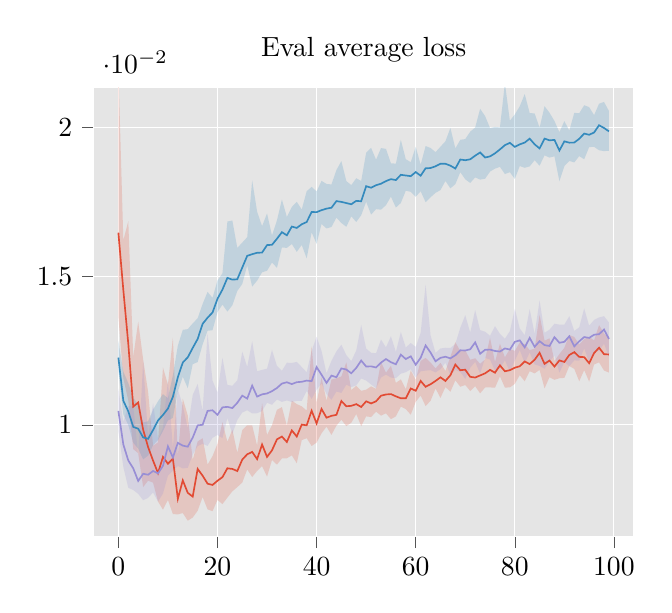
\begin{tikzpicture}

    \definecolor{color0}{rgb}{0.886274509803922,0.290196078431373,0.2}
    \definecolor{color1}{rgb}{0.203921568627451,0.541176470588235,0.741176470588235}
    \definecolor{color2}{rgb}{0.596078431372549,0.556862745098039,0.835294117647059}

    \begin{axis}[
    axis background/.style={fill=white!89.8039215686275!black},
    axis line style={white},
    log basis y={10},
    tick align=outside,
    tick pos=left,
    title={Eval average loss},
    x grid style={white},
    xmajorgrids,
    xmin=-4.95, xmax=103.95,
    xtick style={color=white!33.3333333333333!black},
    y grid style={white},
    ymajorgrids,
%ymin=0.00639289778933677, ymax=0.1,
%ymode=log,
    ytick style={color=white!33.3333333333333!black}
    ]
        \path [fill=color0, fill opacity=0.2, very thin]
        (axis cs:0,0.0219812059283182)
        --(axis cs:0,0.0136346059283182)
        --(axis cs:1,0.011571033442775)
        --(axis cs:2,0.0108228020238203)
        --(axis cs:3,0.00918749532787618)
        --(axis cs:4,0.00904796834822737)
        --(axis cs:5,0.00791150981832493)
        --(axis cs:6,0.00812470593394444)
        --(axis cs:7,0.00806007518128587)
        --(axis cs:8,0.00742376304328255)
        --(axis cs:9,0.00715036971657623)
        --(axis cs:10,0.00747920826037888)
        --(axis cs:11,0.00700225375025664)
        --(axis cs:12,0.00699329118078648)
        --(axis cs:13,0.00703653051063653)
        --(axis cs:14,0.006780136165189)
        --(axis cs:15,0.00688578310950341)
        --(axis cs:16,0.00711500335290847)
        --(axis cs:17,0.00757675626380467)
        --(axis cs:18,0.00716125387606225)
        --(axis cs:19,0.00709967690792966)
        --(axis cs:20,0.00747964328486148)
        --(axis cs:21,0.00733812637535319)
        --(axis cs:22,0.00755708635831057)
        --(axis cs:23,0.00776710024597574)
        --(axis cs:24,0.00790981841401754)
        --(axis cs:25,0.00806237462686794)
        --(axis cs:26,0.008503908718872)
        --(axis cs:27,0.00824909594269698)
        --(axis cs:28,0.00845353210267588)
        --(axis cs:29,0.00861431169387362)
        --(axis cs:30,0.00826336519176147)
        --(axis cs:31,0.00882046387024341)
        --(axis cs:32,0.00866499284444845)
        --(axis cs:33,0.00887398884989382)
        --(axis cs:34,0.00887863306527779)
        --(axis cs:35,0.00897674945976416)
        --(axis cs:36,0.00871088223406785)
        --(axis cs:37,0.0094873204725786)
        --(axis cs:38,0.00955491510937649)
        --(axis cs:39,0.00929195727832234)
        --(axis cs:40,0.00940409680562188)
        --(axis cs:41,0.00971754028207285)
        --(axis cs:42,0.00994195708077802)
        --(axis cs:43,0.0096669319919704)
        --(axis cs:44,0.0099767135891235)
        --(axis cs:45,0.0101755408582421)
        --(axis cs:46,0.00996040293852643)
        --(axis cs:47,0.0100718093238584)
        --(axis cs:48,0.0103666924572954)
        --(axis cs:49,0.00995976670937719)
        --(axis cs:50,0.0102883975964039)
        --(axis cs:51,0.0102646070848296)
        --(axis cs:52,0.0104451063175862)
        --(axis cs:53,0.0103131799234318)
        --(axis cs:54,0.0103898103093629)
        --(axis cs:55,0.0101946421680638)
        --(axis cs:56,0.0102871920835135)
        --(axis cs:57,0.0106146728558447)
        --(axis cs:58,0.0105311447863983)
        --(axis cs:59,0.010344543370805)
        --(axis cs:60,0.0107758269949164)
        --(axis cs:61,0.0109874497136172)
        --(axis cs:62,0.0106335482169102)
        --(axis cs:63,0.0108126294780802)
        --(axis cs:64,0.0112264335838859)
        --(axis cs:65,0.0109077106058246)
        --(axis cs:66,0.0112751622633278)
        --(axis cs:67,0.0111155700422184)
        --(axis cs:68,0.0114987231729766)
        --(axis cs:69,0.0112831800855152)
        --(axis cs:70,0.0113432639535221)
        --(axis cs:71,0.0111401219981791)
        --(axis cs:72,0.0113015851199256)
        --(axis cs:73,0.0110620840584441)
        --(axis cs:74,0.0112582286895705)
        --(axis cs:75,0.0112621218135889)
        --(axis cs:76,0.0112495729901917)
        --(axis cs:77,0.011633091572384)
        --(axis cs:78,0.0112569383738299)
        --(axis cs:79,0.0112600891011014)
        --(axis cs:80,0.01138151282217)
        --(axis cs:81,0.0116716557716029)
        --(axis cs:82,0.0114677157549898)
        --(axis cs:83,0.0118077187279785)
        --(axis cs:84,0.0117321984039295)
        --(axis cs:85,0.0118527368906346)
        --(axis cs:86,0.0112283289232015)
        --(axis cs:87,0.0116041548979595)
        --(axis cs:88,0.0115168318812142)
        --(axis cs:89,0.0115696860400726)
        --(axis cs:90,0.0115815409267675)
        --(axis cs:91,0.0119787139303531)
        --(axis cs:92,0.0118835249271358)
        --(axis cs:93,0.0114675175474394)
        --(axis cs:94,0.0118434049027369)
        --(axis cs:95,0.0114563595983011)
        --(axis cs:96,0.0120338192024621)
        --(axis cs:97,0.0121024692679375)
        --(axis cs:98,0.0118306360809255)
        --(axis cs:99,0.0117596826035947)
        --(axis cs:99,0.0129139826035947)
        --(axis cs:99,0.0129139826035947)
        --(axis cs:98,0.0130800360809255)
        --(axis cs:97,0.0133566692679375)
        --(axis cs:96,0.0128441192024622)
        --(axis cs:95,0.0129567595983011)
        --(axis cs:94,0.0128839049027369)
        --(axis cs:93,0.0127045175474394)
        --(axis cs:92,0.0129579249271358)
        --(axis cs:91,0.0130230139303531)
        --(axis cs:90,0.0125932409267675)
        --(axis cs:89,0.0123839860400726)
        --(axis cs:88,0.0121479318812142)
        --(axis cs:87,0.0129117548979595)
        --(axis cs:86,0.0128312289232015)
        --(axis cs:85,0.0136968368906346)
        --(axis cs:84,0.0125647984039295)
        --(axis cs:83,0.0125147187279785)
        --(axis cs:82,0.0127171157549898)
        --(axis cs:81,0.0127713557716029)
        --(axis cs:80,0.01248881282217)
        --(axis cs:79,0.0125536891011014)
        --(axis cs:78,0.0122735383738299)
        --(axis cs:77,0.012731491572384)
        --(axis cs:76,0.0121189729901917)
        --(axis cs:75,0.0129297218135889)
        --(axis cs:74,0.0122027286895705)
        --(axis cs:73,0.0120546840584441)
        --(axis cs:72,0.0122423851199256)
        --(axis cs:71,0.0121900219981791)
        --(axis cs:70,0.0125135639535221)
        --(axis cs:69,0.0124844800855152)
        --(axis cs:68,0.0127806231729766)
        --(axis cs:67,0.0122928700422184)
        --(axis cs:66,0.0118115622633278)
        --(axis cs:65,0.0120900106058246)
        --(axis cs:64,0.0119017335838859)
        --(axis cs:63,0.0120971294780802)
        --(axis cs:62,0.0122532482169102)
        --(axis cs:61,0.0121530497136172)
        --(axis cs:60,0.0115221269949164)
        --(axis cs:59,0.011833443370805)
        --(axis cs:58,0.0111988447863983)
        --(axis cs:57,0.0115301728558447)
        --(axis cs:56,0.0114146920835135)
        --(axis cs:55,0.0119868421680638)
        --(axis cs:54,0.0117554103093629)
        --(axis cs:53,0.0121145799234318)
        --(axis cs:52,0.0112129063175862)
        --(axis cs:51,0.0112973070848296)
        --(axis cs:50,0.0111856975964039)
        --(axis cs:49,0.0111463067093772)
        --(axis cs:48,0.0113144924572954)
        --(axis cs:47,0.0111735093238584)
        --(axis cs:46,0.0121044729385264)
        --(axis cs:45,0.0116306408582421)
        --(axis cs:44,0.0115676235891235)
        --(axis cs:43,0.0115254019919704)
        --(axis cs:42,0.010813807080778)
        --(axis cs:41,0.0115971502820728)
        --(axis cs:40,0.0107450868056219)
        --(axis cs:39,0.0126469172783223)
        --(axis cs:38,0.0104827351093765)
        --(axis cs:37,0.0106252004725786)
        --(axis cs:36,0.0107001022340678)
        --(axis cs:35,0.0108165594597642)
        --(axis cs:34,0.00997475306527779)
        --(axis cs:33,0.0105986088498938)
        --(axis cs:32,0.0105085128444485)
        --(axis cs:31,0.00998896387024341)
        --(axis cs:30,0.00965785519176147)
        --(axis cs:29,0.0107312216938736)
        --(axis cs:28,0.00930390210267588)
        --(axis cs:27,0.00998562594269698)
        --(axis cs:26,0.009988478718872)
        --(axis cs:25,0.00982318462686794)
        --(axis cs:24,0.00906335841401754)
        --(axis cs:23,0.00984253024597574)
        --(axis cs:22,0.00943341635831057)
        --(axis cs:21,0.0100909163753532)
        --(axis cs:20,0.00936661328486148)
        --(axis cs:19,0.00895413690792966)
        --(axis cs:18,0.00866581387606225)
        --(axis cs:17,0.00955409626380467)
        --(axis cs:16,0.00944467335290847)
        --(axis cs:15,0.00882108310950342)
        --(axis cs:14,0.010316936165189)
        --(axis cs:13,0.0108834205106365)
        --(axis cs:12,0.00897432118078648)
        --(axis cs:11,0.0129371537502566)
        --(axis cs:10,0.0113524482603789)
        --(axis cs:9,0.0119327197165762)
        --(axis cs:8,0.00941406304328255)
        --(axis cs:7,0.00929845518128587)
        --(axis cs:6,0.0111082259339444)
        --(axis cs:5,0.0121987798183249)
        --(axis cs:4,0.0134717783482274)
        --(axis cs:3,0.0122797853278762)
        --(axis cs:2,0.0168506020238203)
        --(axis cs:1,0.016203033442775)
        --(axis cs:0,0.0219812059283182)
        --cycle;

        \path [fill=color1, fill opacity=0.2, very thin]
        (axis cs:0,0.0128194059283182)
        --(axis cs:0,0.0118030059283182)
        --(axis cs:1,0.010353033442775)
        --(axis cs:2,0.00999397202382026)
        --(axis cs:3,0.00940208532787618)
        --(axis cs:4,0.00919932834822737)
        --(axis cs:5,0.00884367981832493)
        --(axis cs:6,0.00896640593394444)
        --(axis cs:7,0.00931708518128587)
        --(axis cs:8,0.00948923304328255)
        --(axis cs:9,0.00979439971657623)
        --(axis cs:10,0.0101511482603789)
        --(axis cs:11,0.0102357537502566)
        --(axis cs:12,0.0111258511807865)
        --(axis cs:13,0.0116198205106365)
        --(axis cs:14,0.011235736165189)
        --(axis cs:15,0.0120415731095034)
        --(axis cs:16,0.0121126433529085)
        --(axis cs:17,0.0127083062638047)
        --(axis cs:18,0.0131652238760622)
        --(axis cs:19,0.0131845069079297)
        --(axis cs:20,0.0137910832848615)
        --(axis cs:21,0.0140457163753532)
        --(axis cs:22,0.0138100063583106)
        --(axis cs:23,0.0140201102459757)
        --(axis cs:24,0.0145042684140175)
        --(axis cs:25,0.0147389146268679)
        --(axis cs:26,0.015359028718872)
        --(axis cs:27,0.014650315942697)
        --(axis cs:28,0.0148514021026759)
        --(axis cs:29,0.0151301216938736)
        --(axis cs:30,0.0151833151917615)
        --(axis cs:31,0.0154589338702434)
        --(axis cs:32,0.0152822128444485)
        --(axis cs:33,0.0159664088498938)
        --(axis cs:34,0.0159508030652778)
        --(axis cs:35,0.0160820594597642)
        --(axis cs:36,0.0158192022340678)
        --(axis cs:37,0.0160509004725786)
        --(axis cs:38,0.0155998351093765)
        --(axis cs:39,0.0164740172783223)
        --(axis cs:40,0.0160880868056219)
        --(axis cs:41,0.0167544502820728)
        --(axis cs:42,0.016605907080778)
        --(axis cs:43,0.0166532019919704)
        --(axis cs:44,0.0169683235891235)
        --(axis cs:45,0.0167885408582421)
        --(axis cs:46,0.0166614729385264)
        --(axis cs:47,0.0170116093238584)
        --(axis cs:48,0.0168226924572954)
        --(axis cs:49,0.0170480067093772)
        --(axis cs:50,0.0175006975964039)
        --(axis cs:51,0.0170699070848296)
        --(axis cs:52,0.0172541063175862)
        --(axis cs:53,0.0172366799234318)
        --(axis cs:54,0.0173874103093629)
        --(axis cs:55,0.0176742421680638)
        --(axis cs:56,0.0173079920835135)
        --(axis cs:57,0.0174616728558447)
        --(axis cs:58,0.0178740447863983)
        --(axis cs:59,0.017836643370805)
        --(axis cs:60,0.0176701269949164)
        --(axis cs:61,0.0178552497136172)
        --(axis cs:62,0.0174881482169102)
        --(axis cs:63,0.0176530294780802)
        --(axis cs:64,0.0178016335838859)
        --(axis cs:65,0.0178951106058246)
        --(axis cs:66,0.0182002622633278)
        --(axis cs:67,0.0179540700422184)
        --(axis cs:68,0.0180927231729766)
        --(axis cs:69,0.0184965800855152)
        --(axis cs:70,0.0182577639535221)
        --(axis cs:71,0.0181351219981791)
        --(axis cs:72,0.0183214851199256)
        --(axis cs:73,0.0182468840584441)
        --(axis cs:74,0.0182761286895705)
        --(axis cs:75,0.0185159218135889)
        --(axis cs:76,0.0186161729901917)
        --(axis cs:77,0.018674491572384)
        --(axis cs:78,0.0184346383738299)
        --(axis cs:79,0.0184970891011014)
        --(axis cs:80,0.01827011282217)
        --(axis cs:81,0.0187028557716029)
        --(axis cs:82,0.0186442157549898)
        --(axis cs:83,0.0186913187279785)
        --(axis cs:84,0.0188975984039295)
        --(axis cs:85,0.0187138368906346)
        --(axis cs:86,0.0190621289232015)
        --(axis cs:87,0.0189869548979595)
        --(axis cs:88,0.0190296318812142)
        --(axis cs:89,0.0181915860400726)
        --(axis cs:90,0.0187000409267675)
        --(axis cs:91,0.0188746139303531)
        --(axis cs:92,0.0188250249271358)
        --(axis cs:93,0.0190369175474394)
        --(axis cs:94,0.0189292049027369)
        --(axis cs:95,0.0193399595983011)
        --(axis cs:96,0.0193489192024621)
        --(axis cs:97,0.0192332692679375)
        --(axis cs:98,0.0192046360809255)
        --(axis cs:99,0.0192178826035947)
        --(axis cs:99,0.0205530826035947)
        --(axis cs:99,0.0205530826035947)
        --(axis cs:98,0.0208591360809255)
        --(axis cs:97,0.0207995692679375)
        --(axis cs:96,0.0204157192024622)
        --(axis cs:95,0.0206842595983011)
        --(axis cs:94,0.0207476049027369)
        --(axis cs:93,0.0204783175474394)
        --(axis cs:92,0.0204928249271358)
        --(axis cs:91,0.0198946139303531)
        --(axis cs:90,0.0202135409267675)
        --(axis cs:89,0.0198435860400726)
        --(axis cs:88,0.0202174318812142)
        --(axis cs:87,0.0204978548979595)
        --(axis cs:86,0.0207149289232015)
        --(axis cs:85,0.0199913368906346)
        --(axis cs:84,0.0204713984039295)
        --(axis cs:83,0.0204867187279785)
        --(axis cs:82,0.0211230157549898)
        --(axis cs:81,0.0207130557716029)
        --(axis cs:80,0.02043881282217)
        --(axis cs:79,0.0202269891011014)
        --(axis cs:78,0.0214923383738299)
        --(axis cs:77,0.020002891572384)
        --(axis cs:76,0.0200169729901917)
        --(axis cs:75,0.0199837218135889)
        --(axis cs:74,0.0203840286895705)
        --(axis cs:73,0.0206279840584441)
        --(axis cs:72,0.0199976851199256)
        --(axis cs:71,0.0198581219981791)
        --(axis cs:70,0.0196105639535221)
        --(axis cs:69,0.0195850800855152)
        --(axis cs:68,0.0192967231729766)
        --(axis cs:67,0.0199856700422184)
        --(axis cs:66,0.0195366622633278)
        --(axis cs:65,0.0193542106058246)
        --(axis cs:64,0.0191710335838859)
        --(axis cs:63,0.0193114294780802)
        --(axis cs:62,0.0193756482169102)
        --(axis cs:61,0.0187499497136172)
        --(axis cs:60,0.0193486269949164)
        --(axis cs:59,0.018833743370805)
        --(axis cs:58,0.0189336447863983)
        --(axis cs:57,0.0195831728558447)
        --(axis cs:56,0.0187827920835135)
        --(axis cs:55,0.0187970421680638)
        --(axis cs:54,0.0192793103093629)
        --(axis cs:53,0.0193081799234318)
        --(axis cs:52,0.0189198063175862)
        --(axis cs:51,0.0193134070848296)
        --(axis cs:50,0.0191506975964039)
        --(axis cs:49,0.0182011067093772)
        --(axis cs:48,0.0182933924572954)
        --(axis cs:47,0.0180628093238584)
        --(axis cs:46,0.0181989729385264)
        --(axis cs:45,0.0188712408582421)
        --(axis cs:44,0.0185690235891235)
        --(axis cs:43,0.0180851019919704)
        --(axis cs:42,0.018101007080778)
        --(axis cs:41,0.0182058502820728)
        --(axis cs:40,0.0178494868056219)
        --(axis cs:39,0.0180034172783223)
        --(axis cs:38,0.0178578351093765)
        --(axis cs:37,0.0172418004725786)
        --(axis cs:36,0.0175025022340679)
        --(axis cs:35,0.0173278594597642)
        --(axis cs:34,0.0169929030652778)
        --(axis cs:33,0.0175812088498938)
        --(axis cs:32,0.0168769128444485)
        --(axis cs:31,0.0163697338702434)
        --(axis cs:30,0.0171102151917615)
        --(axis cs:29,0.0166834216938736)
        --(axis cs:28,0.0171671021026759)
        --(axis cs:27,0.018223915942697)
        --(axis cs:26,0.016312228718872)
        --(axis cs:25,0.0161315146268679)
        --(axis cs:24,0.0159510684140175)
        --(axis cs:23,0.0168731102459757)
        --(axis cs:22,0.0168400063583106)
        --(axis cs:21,0.0150958163753532)
        --(axis cs:20,0.0148574832848615)
        --(axis cs:19,0.0142709069079297)
        --(axis cs:18,0.0144737238760622)
        --(axis cs:17,0.0140667062638047)
        --(axis cs:16,0.0135869433529085)
        --(axis cs:15,0.0134132731095034)
        --(axis cs:14,0.013221336165189)
        --(axis cs:13,0.0131968205106365)
        --(axis cs:12,0.0126672511807865)
        --(axis cs:11,0.0116705537502566)
        --(axis cs:10,0.0108995482603789)
        --(axis cs:9,0.0110350197165762)
        --(axis cs:8,0.0107971130432826)
        --(axis cs:7,0.0105119051812859)
        --(axis cs:6,0.0101228259339444)
        --(axis cs:5,0.0100811798183249)
        --(axis cs:4,0.0106787783482274)
        --(axis cs:3,0.0109237853278762)
        --(axis cs:2,0.0114078020238203)
        --(axis cs:1,0.011788933442775)
        --(axis cs:0,0.0128194059283182)
        --cycle;

        \path [fill=color2, fill opacity=0.2, very thin]
        (axis cs:0,0.0112171589283182)
        --(axis cs:0,0.00978173982831818)
        --(axis cs:1,0.00858494514277504)
        --(axis cs:2,0.00788492052382026)
        --(axis cs:3,0.00781247052787618)
        --(axis cs:4,0.00768326214822737)
        --(axis cs:5,0.00746807751832493)
        --(axis cs:6,0.00754785913394444)
        --(axis cs:7,0.00772705428128587)
        --(axis cs:8,0.00742400214328255)
        --(axis cs:9,0.00769179671657623)
        --(axis cs:10,0.00829239226037888)
        --(axis cs:11,0.00845882735025664)
        --(axis cs:12,0.00861857098078648)
        --(axis cs:13,0.00853665191063653)
        --(axis cs:14,0.008557944565189)
        --(axis cs:15,0.00899768190950341)
        --(axis cs:16,0.00928986245290847)
        --(axis cs:17,0.00936627156380467)
        --(axis cs:18,0.00929548837606225)
        --(axis cs:19,0.00956513210792966)
        --(axis cs:20,0.00966452528486148)
        --(axis cs:21,0.00955385317535319)
        --(axis cs:22,0.0102314177583106)
        --(axis cs:23,0.00969331284597574)
        --(axis cs:24,0.0101664149140175)
        --(axis cs:25,0.0104150690268679)
        --(axis cs:26,0.010493403818872)
        --(axis cs:27,0.010385412042697)
        --(axis cs:28,0.0103934453026759)
        --(axis cs:29,0.0104658088938736)
        --(axis cs:30,0.0107451910917615)
        --(axis cs:31,0.0106770582702434)
        --(axis cs:32,0.0108537698444485)
        --(axis cs:33,0.0107761709498938)
        --(axis cs:34,0.0108224620652778)
        --(axis cs:35,0.0107708093597642)
        --(axis cs:36,0.0108099396340678)
        --(axis cs:37,0.0108058323725786)
        --(axis cs:38,0.0111405533093765)
        --(axis cs:39,0.0108733641783223)
        --(axis cs:40,0.0111825554056219)
        --(axis cs:41,0.0113969713820728)
        --(axis cs:42,0.011036358680778)
        --(axis cs:43,0.0108451113919704)
        --(axis cs:44,0.0111233081891235)
        --(axis cs:45,0.0110754621582421)
        --(axis cs:46,0.0113540003385264)
        --(axis cs:47,0.0112712714238584)
        --(axis cs:48,0.0113271135572954)
        --(axis cs:49,0.0115604271093772)
        --(axis cs:50,0.0114931294964039)
        --(axis cs:51,0.0113598056848296)
        --(axis cs:52,0.0112336142175862)
        --(axis cs:53,0.0115956523234318)
        --(axis cs:54,0.0116900004093629)
        --(axis cs:55,0.0115931490680638)
        --(axis cs:56,0.0115699992835135)
        --(axis cs:57,0.0117231231558447)
        --(axis cs:58,0.0117729413863983)
        --(axis cs:59,0.011870777270805)
        --(axis cs:60,0.0115923868949164)
        --(axis cs:61,0.0118031983136172)
        --(axis cs:62,0.0118255345169102)
        --(axis cs:63,0.0118412982780802)
        --(axis cs:64,0.0117654022838859)
        --(axis cs:65,0.0118737338058246)
        --(axis cs:66,0.0120870188633278)
        --(axis cs:67,0.0116804454422184)
        --(axis cs:68,0.0118508372729766)
        --(axis cs:69,0.0117774129855152)
        --(axis cs:70,0.0115511647535221)
        --(axis cs:71,0.0119213748981791)
        --(axis cs:72,0.0121213787199256)
        --(axis cs:73,0.0117237376584441)
        --(axis cs:74,0.0122541064895705)
        --(axis cs:75,0.0121982199135889)
        --(axis cs:76,0.0118208813901917)
        --(axis cs:77,0.011896827072384)
        --(axis cs:78,0.0121708048738299)
        --(axis cs:79,0.0117876363011014)
        --(axis cs:80,0.01215892722217)
        --(axis cs:81,0.0125149689716029)
        --(axis cs:82,0.0120798632549898)
        --(axis cs:83,0.0124372603279785)
        --(axis cs:84,0.0120328267039295)
        --(axis cs:85,0.0119838842906346)
        --(axis cs:86,0.0118881340232015)
        --(axis cs:87,0.0121343100979595)
        --(axis cs:88,0.0123354883812142)
        --(axis cs:89,0.0117573026400726)
        --(axis cs:90,0.0121122605267675)
        --(axis cs:91,0.0119749721303531)
        --(axis cs:92,0.0121699037271358)
        --(axis cs:93,0.0121590204474394)
        --(axis cs:94,0.0125723657027369)
        --(axis cs:95,0.0121220640983011)
        --(axis cs:96,0.0124595616024622)
        --(axis cs:97,0.0124828731679375)
        --(axis cs:98,0.0127319211809255)
        --(axis cs:99,0.0122820800035947)
        --(axis cs:99,0.0134442943035947)
        --(axis cs:99,0.0134442943035947)
        --(axis cs:98,0.0136560276809255)
        --(axis cs:97,0.0136134887679375)
        --(axis cs:96,0.0135295448024621)
        --(axis cs:95,0.0133380584983011)
        --(axis cs:94,0.0139204907027369)
        --(axis cs:93,0.0132823927474394)
        --(axis cs:92,0.0131594904271358)
        --(axis cs:91,0.0136559089303531)
        --(axis cs:90,0.0133735563267675)
        --(axis cs:89,0.0133738761400726)
        --(axis cs:88,0.0134020162812142)
        --(axis cs:87,0.0132028511979595)
        --(axis cs:86,0.0131000253232015)
        --(axis cs:85,0.0141872872906346)
        --(axis cs:84,0.0130613971039295)
        --(axis cs:83,0.0138926339279785)
        --(axis cs:82,0.0130150414549898)
        --(axis cs:81,0.0132446929716029)
        --(axis cs:80,0.01390695182217)
        --(axis cs:79,0.0131536275011014)
        --(axis cs:78,0.0128978305738299)
        --(axis cs:77,0.013063408572384)
        --(axis cs:76,0.0133200479901917)
        --(axis cs:75,0.0129976965135889)
        --(axis cs:74,0.0131350050895705)
        --(axis cs:73,0.0131884730584441)
        --(axis cs:72,0.0138617963199256)
        --(axis cs:71,0.0131072903981791)
        --(axis cs:70,0.0136886980535221)
        --(axis cs:69,0.0132682430855152)
        --(axis cs:68,0.0127224390729766)
        --(axis cs:67,0.0125864631422184)
        --(axis cs:66,0.0125950522633278)
        --(axis cs:65,0.0125701177058246)
        --(axis cs:64,0.0124243767838859)
        --(axis cs:63,0.0130068029780802)
        --(axis cs:62,0.0147171473169102)
        --(axis cs:61,0.0130971236136172)
        --(axis cs:60,0.0126234562949164)
        --(axis cs:59,0.012753897270805)
        --(axis cs:58,0.0126049078863983)
        --(axis cs:57,0.0131263966558447)
        --(axis cs:56,0.0124587926835135)
        --(axis cs:55,0.0129815959680638)
        --(axis cs:54,0.0126074828093629)
        --(axis cs:53,0.0128705449234318)
        --(axis cs:52,0.0124103793175862)
        --(axis cs:51,0.0124262544848296)
        --(axis cs:50,0.0125679692964039)
        --(axis cs:49,0.0133635564093772)
        --(axis cs:48,0.0125030517572954)
        --(axis cs:47,0.0121462852238584)
        --(axis cs:46,0.0123477570385264)
        --(axis cs:45,0.0126987950582421)
        --(axis cs:44,0.0124728287891235)
        --(axis cs:43,0.0121555047919704)
        --(axis cs:42,0.011736421680778)
        --(axis cs:41,0.0124880158820728)
        --(axis cs:40,0.0129645432056219)
        --(axis cs:39,0.0124943935783223)
        --(axis cs:38,0.0117705622093765)
        --(axis cs:37,0.0119477768725786)
        --(axis cs:36,0.0121182883340678)
        --(axis cs:35,0.0120842162597642)
        --(axis cs:34,0.0120928115652778)
        --(axis cs:33,0.0118205399498938)
        --(axis cs:32,0.0119834654444485)
        --(axis cs:31,0.0125217312702434)
        --(axis cs:30,0.0118912072917615)
        --(axis cs:29,0.0118511833938736)
        --(axis cs:28,0.0118038570026759)
        --(axis cs:27,0.012814553242697)
        --(axis cs:26,0.011957169818872)
        --(axis cs:25,0.0124618858268679)
        --(axis cs:24,0.0114997166140175)
        --(axis cs:23,0.0113163033459757)
        --(axis cs:22,0.0113454674583106)
        --(axis cs:21,0.0122571585753532)
        --(axis cs:20,0.0110894484848615)
        --(axis cs:19,0.0114890232079297)
        --(axis cs:18,0.0130781288760622)
        --(axis cs:17,0.0104682446638047)
        --(axis cs:16,0.0113803869529085)
        --(axis cs:15,0.0110078156095034)
        --(axis cs:14,0.009888894965189)
        --(axis cs:13,0.0106465328106365)
        --(axis cs:12,0.0112056257807865)
        --(axis cs:11,0.00923211665025664)
        --(axis cs:10,0.0114868129603789)
        --(axis cs:9,0.00989519461657623)
        --(axis cs:8,0.00952286644328255)
        --(axis cs:7,0.0107327125812859)
        --(axis cs:6,0.00957582953394444)
        --(axis cs:5,0.0121353525183249)
        --(axis cs:4,0.00895266784822737)
        --(axis cs:3,0.0106394727278762)
        --(axis cs:2,0.0106341414238203)
        --(axis cs:1,0.010107984542775)
        --(axis cs:0,0.0112171589283182)
        --cycle;

        \addplot [semithick, color0]
        table {%
        0 0.0164623633027077
        1 0.014535877853632
        2 0.0127287125214934
        3 0.0106151672080159
        4 0.0107560325413942
        5 0.00983761623501778
        6 0.00925472844392061
        7 0.00880009960383177
        8 0.0083821527659893
        9 0.00892423093318939
        10 0.00869645550847054
        11 0.0088665634393692
        12 0.0075157736428082
        13 0.00813695043325424
        14 0.00771807273849845
        15 0.00759043078869581
        16 0.00852066185325384
        17 0.00829320959746838
        18 0.00802520103752613
        19 0.007982412353158
        20 0.00812419783324003
        21 0.00824433378875256
        22 0.00854289997369051
        23 0.00852040015161037
        24 0.00845058541744947
        25 0.00883457344025373
        26 0.00901274103671312
        27 0.009093027561903
        28 0.00885113701224327
        29 0.00933993980288506
        30 0.00892546586692333
        31 0.00914660841226578
        32 0.00951564777642488
        33 0.00960901007056236
        34 0.00942611694335938
        35 0.00981506239622831
        36 0.00960990693420172
        37 0.0100109744817019
        38 0.00998758990317583
        39 0.0104787927120924
        40 0.0100506199523807
        41 0.0105365607887506
        42 0.0102438619360328
        43 0.0103055639192462
        44 0.0103392219170928
        45 0.0108032617717981
        46 0.0106284208595753
        47 0.0106421653181314
        48 0.0106994835659862
        49 0.0106040798127651
        50 0.0107942745089531
        51 0.0107231633737683
        52 0.0107946721836925
        53 0.0109820459038019
        54 0.0110240094363689
        55 0.0110369650647044
        56 0.01096111536026
        57 0.0108959609642625
        58 0.0108947111293674
        59 0.0112262303009629
        60 0.0111497053876519
        61 0.0114786392077804
        62 0.0112829590216279
        63 0.011369239538908
        64 0.0114798014983535
        65 0.0116004338487983
        66 0.0114791179075837
        67 0.0116715915501118
        68 0.012029723264277
        69 0.0118400566279888
        70 0.0118564739823341
        71 0.0116178002208471
        72 0.0115939751267433
        74 0.0117345508188009
        75 0.0118511207401752
        76 0.0117563614621758
        77 0.0120028015226126
        78 0.0118038840591908
        79 0.0118410671129823
        80 0.0119245890527964
        81 0.011972145177424
        82 0.0121343610808253
        83 0.0120460530743003
        84 0.0121904769912362
        85 0.0124241933226585
        86 0.0120531311258674
        87 0.0121640115976334
        88 0.0119632659479976
        89 0.0121682090684772
        90 0.0121179083362222
        91 0.0123529257252812
        92 0.0124459806829691
        93 0.0122878830879927
        94 0.0122789954766631
        95 0.0120758153498173
        96 0.0124159194529057
        97 0.0125970114022493
        98 0.0123792449012399
        99 0.0123688383027911
        };
        \addplot [semithick, color1]
        table {%
        0 0.012265507131815
        1 0.0108121139928699
        2 0.0104576209560037
        3 0.00993480253964663
        4 0.0098732765763998
        5 0.00958023499697447
        6 0.00953339971601963
        7 0.00982919987291098
        8 0.0101500609889627
        9 0.0103360181674361
        10 0.0105501487851143
        11 0.0109446039423347
        12 0.0116023505106568
        13 0.0120989605784416
        14 0.0122726568952203
        15 0.0125876720994711
        16 0.0128912646323442
        17 0.0133981667459011
        18 0.0136049827560782
        19 0.013779629021883
        20 0.0142410043627024
        21 0.0145493056625128
        22 0.0149436062201858
        23 0.0148842306807637
        24 0.0148969180881977
        26 0.0156847201287746
        27 0.015739968046546
        28 0.0157876294106245
        29 0.0157940704375505
        30 0.0160460863262415
        31 0.016055703163147
        32 0.0162587352097034
        33 0.016479728743434
        34 0.0163752026855946
        35 0.0166687294840813
        36 0.0166232623159885
        37 0.0167461317032576
        38 0.0168212242424488
        39 0.017158905044198
        40 0.0171533152461052
        41 0.0172201301902533
        42 0.0172717049717903
        43 0.0173021927475929
        44 0.0175243224948645
        45 0.0174983534961939
        47 0.0174188986420631
        48 0.0175323821604252
        49 0.0175197590142488
        50 0.0180267058312893
        51 0.0179745685309172
        52 0.0180588569492102
        53 0.0181094892323017
        54 0.0181978326290846
        55 0.0182630848139524
        56 0.0182318110018969
        57 0.0184093210846186
        59 0.0183623917400837
        60 0.0185018796473742
        61 0.0183777920901775
        62 0.0186267700046301
        63 0.0186364874243736
        64 0.0186956450343132
        65 0.0187794528901577
        66 0.0187795516103506
        67 0.0187171902507544
        68 0.0186194553971291
        69 0.0189230497926474
        70 0.0188987050205469
        71 0.0189301408827305
        72 0.0190520323812962
        73 0.0191597826778889
        74 0.018990371376276
        75 0.0190281793475151
        76 0.019130764529109
        77 0.0192623641341925
        78 0.0194050874561071
        79 0.0194838605821133
        80 0.0193473324179649
        81 0.0194331984966993
        82 0.0194919258356094
        83 0.0196240171790123
        84 0.0194336678832769
        85 0.019294885918498
        86 0.0196263715624809
        87 0.0195677857846022
        88 0.0195816494524479
        89 0.0192265268415213
        90 0.0195340309292078
        91 0.019488861784339
        92 0.019492756575346
        93 0.019619757309556
        94 0.0197951532900333
        95 0.0197549518197775
        96 0.0198314599692822
        97 0.0200753100216389
        98 0.0199828371405602
        99 0.0198687016963959
        };
        \addplot [semithick, color2]
        table {%
        0 0.0104707879945636
        1 0.00934168789535761
        2 0.00880510546267033
        3 0.00854012463241816
        4 0.00811731908470392
        5 0.00835807994008064
        6 0.00832660775631666
        7 0.00845173094421625
        8 0.00837122183293104
        9 0.0086278123781085
        10 0.00928199011832476
        11 0.00890406407415867
        12 0.00939653813838959
        13 0.00930392742156982
        14 0.00926866475492716
        15 0.0095748407766223
        16 0.00998560525476933
        17 0.0100050214678049
        18 0.0104716587811708
        19 0.010492536239326
        20 0.0103395935148001
        21 0.010590111836791
        22 0.010607972741127
        23 0.0105671286582947
        24 0.0107432501390576
        25 0.0109846089035273
        26 0.0108853755518794
        27 0.011321977712214
        28 0.0109522771090269
        29 0.0110288485884666
        30 0.0110571049153805
        31 0.011135776527226
        32 0.0112420283257961
        33 0.0113903991878033
        34 0.0114347599446774
        35 0.0113733997568488
        36 0.0114373406395316
        37 0.011449933052063
        38 0.0114915110170841
        39 0.0114713124930859
        40 0.0119442967697978
        41 0.0116871017962694
        42 0.0114142009988427
        43 0.011658332310617
        44 0.0116052869707346
        45 0.0119000785052776
        46 0.0118625508621335
        47 0.0117373764514923
        48 0.0119169456884265
        49 0.0121640916913748
        50 0.0119635844603181
        51 0.0119699304923415
        52 0.0119313271716237
        53 0.0120953246951103
        54 0.0122145293280482
        55 0.012109249830246
        56 0.0120397489517927
        57 0.0123623181134462
        58 0.0122147239744663
        59 0.0123057318851352
        60 0.0120247714221478
        61 0.0122568579390645
        62 0.0126719838008285
        63 0.012432855553925
        64 0.0121405115351081
        65 0.0122552867978811
        66 0.0122929904609919
        67 0.0122383404523134
        68 0.0123432893306017
        69 0.0125090749934316
        70 0.0125031294301152
        71 0.0125431064516306
        72 0.0127746565267444
        73 0.012393195182085
        74 0.0125256767496467
        75 0.0125328376889229
        76 0.0124868312850595
        77 0.0124675426632166
        78 0.0125721469521523
        79 0.0125330062583089
        80 0.0127943083643913
        81 0.0128427762538195
        82 0.0126073956489563
        83 0.0129254534840584
        84 0.012626918964088
        85 0.0128165502101183
        86 0.012683192268014
        87 0.0126547114923596
        88 0.0129501027986407
        89 0.0127614475786686
        90 0.0127942133694887
        91 0.012981079518795
        92 0.0126430001109838
        93 0.0128120519220829
        94 0.0129543403163552
        95 0.0129250809550285
        96 0.0130329988896847
        97 0.013050751760602
        98 0.0132067175582051
        99 0.0128922024741769
        };
    \end{axis}

\end{tikzpicture}
;
        \end{adjustbox}
    \end{subfigure}
    \caption{Comparison of PyTorch, LibTorch, and cuDNN implementations on CIFAR10.}
    \label{fig:teaser}
\end{teaserfigure}
